\documentclass[final,fmstyle]{./util/ucathesis}
% La opcion 'final' muestra los graficos, para generar una version sin los graficos utiliza la opcion 'draft'

% paquetes recomendados
%\usepackage[chapter]{theorems}
%\usepackage{symbols}
%\usepackage{url}
\usepackage{amsmath,amsthm}
\usepackage{textcomp}
\usepackage[T1]{fontenc}
\usepackage[spanish]{babel}
\usepackage[utf8]{inputenc}
\usepackage{csquotes}
\usepackage{enumerate}
\usepackage{enumitem}
\usepackage[style=authoryear, uniquename=full, sorting=none,backend=biber, natbib=true]{biblatex}
\usepackage{listings}
% para la lista de simbolos
\usepackage{array} %for vertical thick lines in tables
\usepackage{multirow} %multirow tables
\usepackage{nicefrac} %for fractions like 1/4
% para las tablas
\usepackage{tablefootnote}
\renewcommand{\thefootnote}{\arabic{footnote}}
%referencias
\addbibresource{referencias.bib}
%Package list ends here

% Macro for 'List of Symbols', 'List of Notations' etc...
\def\listofsymbols{
    \newpage
\chapter*{Lista de Símbolos\hfill}
\addcontentsline{toc}{chapter}{Lista de Símbolos}
\begin{tabbing}
% YOU NEED TO ADD THE FIRST ONE MANUALLY TO ADJUST THE TABBING AND SPACES
$n$~~~~~~~~~~\=\parbox{5in}{Vector size\dotfill \pageref{symbol:nml}}\\
%ADD THE REST OF SYMBOLS WITH THE HELP OF MACRO

%% se añaden nuevos simbolos con el macro \newsymbol y se hace referecnia
% al simbolo utilizando \addsymbol{symbol:LABEL}

%\newsymbol (x_i, y_i): {coordenadas que representan un punto}{symbol:xy_i}

\end{tabbing}

    \clearpage{}
}
\def\newsymbol #1: #2#3{$#1$ \> \parbox{5in}{#2 \dotfill \pageref{#3}}\\}
\def\addsymbol#1{\label{#1}}

% custom commands
\newcommand{\foreign}[1]{{\it #1}}
\DeclareMathOperator*{\argmax}{arg\,max}
\algsetup{indent=2em}

% \setcounter{tocdepth}{3}

% datos de la tesis
\title{Modelo predictivo de focos de dengue aplicado a Sistemas de informaci\'on geogr\'afica}
\author{Maximiliano B\'{a}ez Gonz\'{a}lez y Roberto Ba\~{n}uelos}
\degree{Inform\'{a}tica}

\advisor{Prof. MSc.}{Guillermo Gonz\'{a}lez}

%\newtheorem{definicion}{Definicin}

\logosource{./graphics/logo.jpg}
\institution{Universidad Nacional de Asunci\'{o}n}
\faculty{Facultad Polit\'{e}cnica}
\address{San Lorenzo - Paraguay}

\begin{document}
\lstset{
    language=java,
    basicstyle=\small\sffamily,
    numbers=left,
    numberstyle=\tiny,
    frame=tb,
    columns=fullflexible,
    showstringspaces=false
}
\maketitle     % esto hace las portadas

% Agradecimientos
%\newpage

\chapter*{\centering Agradecimientos}

A mis padres por haberme brindado la oportunidad de estudiar una carrera Universitaria, por su esfuerzo y entera confianza.

A mis hermanos Alejandra, Mabel, Marcos y Matías gracias la paciencia, por acompañarme siempre en los buenos y malos momentos, por brindarme su apoyo incondicionalmente.

A mi hermano Marcos, gracias por todo el apoyo, la orientación, por iluminar mi camino y darme una pauta para poder realizarme en mis estudios y en la vida, gracias por siempre estar cerca a pesar de la distancia.

A mi tutor Prof. MSc. Guillermo González por encaminar y acompañar el desarrollo este trabajo hasta su culminación, gracias profesor por haber compartido sus conocimientos conmigo y su gran ayuda para lograr esta meta tan importante.

A Lindsay, gracias por siempre estar a mi lado, por acompañarme incondicionalmente, por todos los consejos y por ayudarme a enfrentar y superar los momentos difíciles.

A mis jefes, Ing. Joaquin Lima y Ing. Juan Talavera por brindarme tiempo y espacio para el desarrollo de este proyecto siempre que lo necesité.

A mis amigos y compañeros de clases, por permitirme compartir toda esta etapa de formación académica, humana y profesional, gracias por todos los buenos momentos dentro y fuera de las aulas.




% los siguientes comandos producen 'indices.

% Tabla de contenidos
\tableofcontents
% Lista de figuras
\listoffigures
% Lista de tablas
\listoftables
% Lista de algoritmos
\listofalgorithms
%\include{acronimos}
\listofsymbols


\mainmatter  % inician los capitulos de la tesis

% incluye aqui los capitulos (un archivo .tex por capitulo)
%\chapter{Introducción}
En este capítulo se presentan los antecedentes y la importancia de este trabajo, así como las
propuestas que se realizan con el fin de apoyar la lucha preventiva contra el dengue. Conceptos de
la ecología del vector, método de prevención y sistemas de información geográficos son puntos
vitales de este trabajo por lo que son introducidos brevemente en este capítulo. No obstante, en
capítulos siguientes, se tratarán todos estos temas serán desglosados detalladamente.

\section{Justificación y Antecedentes}

El Dengue es una enfermedad viral transmitida por el mosquito Aedes aegypti y representa un
problema grave para la salud pública a nivel mundial \citep{dengueUruguayCap1, world2009dengue, DIBO2005}. Más de 2 500 millones de personas viven en
zonas en riesgo de dengue y más de 100 países han informado de la presencia de esta enfermedad en
su territorio \cite{world2009dengue, gustavo2006dengue}.

Los sistemas de información geográfica (SIG) constituyen un área de rápido desarrollo dentro
de la informática y ofrecen métodos sumamente innovadores para hacer frente a algunas demandas
técnicas que constituyen un reto. Un sistema de información geográfica es una integración
organizada de hardware, software, datos geográficos y personal, diseñado para capturar, almacenar,
manipular, analizar y visualizar en todas sus formas la información geográficamente referenciada
con el fin de resolver problemas complejos de planificación y gestión \citep{lopezMarcos2007}.

Las autoridades sanitarias, en sus tareas de vigilancia en Salud Pública, tienen en los SIG una
herramienta fundamental para conocer cómo se extiende una enfermedad, estudiar su posible relación
con un potencial foco de riesgo, o localizar un brote epidémico \citep{vgomesAegis2001}.

Actualmente el dengue es catalogado como ejemplo de una enfermedad que puede constituir una
emergencia de salud pública de interés internacional con implicaciones para la seguridad
sanitaria \citep{dengueUruguayCap1, world2009dengue}, debido a la necesidad de interrumpir la infección y la rápida propagación de la
epidemia más allá de las fronteras.

Debido a una lucha no efectiva en contra el dengue, en  el Paraguay, cada día se reportan más
nuevos casos de infectados por el dengue. La detección de focos de infección en base a casos
reportados y el combate correctivo realizado actualmente, no resultan efectivos ante la lucha
contra el dengue. Se podrían obtener mejores resultados, realizando un cambio de enfoque, en el
combate contra el dengue, de uno correctivo a uno preventivo.

\section{Propuesta de esta tesis y Objetivos}
En este trabajo se propone la construcción de una herramienta que permita realizar estudios
epidemiológicos de forma cartográfica, especializada para el particular caso del dengue. Se
pretende constituir un modelo que permita predecir los focos de riesgo del dengue, con la ayuda de
un sistema de información geográfica. Para determinar las posibles zonas de riesgo, se debe
construir un algoritmo que permita simular el comportamiento de un mosquito o de un conjunto de
mosquitos de acuerdo a las variables de la región y tener en cuenta sus patrones migratorios.

El objetivo principal es diseñar un modelo y construir una herramienta que permita analizar la
extensión del vector del dengue y estudiar su posible relación con un potencial foco de riesgo, de
forma a realizar una predicción de posibles focos y ayudar a realizar una lucha preventiva contra
la enfermedad. Donde el modelo resultante se pueda aplicar a cualquier región o área de estudio y
que ayude a las autoridades pertinentes para toma de decisiones en la lucha contra el dengue.

\section{Organización del trabajo}
El trabajo está organizado como sigue: el capítulo 2 introduce a los sistemas de información
geográfica, la representación de datos geoespaciales y los métodos de interpolación como
herramienta para análisis espacial. En el capítulo 3 se presenta al aedes aegypti el principal
transmisor del dengue, sus características biológicas y los métodos de muestreo de la abundancia
pobacional del vector. Estos capítulos representan el estado del arte de este trabajo.

El capítulo 4 se presenta el modelo matemático propuesto para la identificación de focos de
infestación y la simulación del proceso evolutivo del ciclo de vida del vector. En el capítulo 5
se presenta la implementación computacional denominada GeoDengue, sus requerimientos, diseño y
arquitectura y las herramientas y tecnologías utilizadas para su implementación.

En el capítulo 6 se presenta los resultados experimentales obtenidos. Finalmente el capítulo 7
presenta las conclusiones de este trabajo y los  posibles trabajos futuros derivados de esta tesis.

%\chapter{Sistemas de Información Geográfica}
Con el transcurrir del tiempo se ha tratado de representar la superficie terrestre y los elementos
que esta alberga. Los primeros mapas, que no presentaban un alto grado de exactitud, eran
utilizados como herramienta para la navegación. Con el paso del tiempo los requerimientos fueron
creciendo, surgiendo así la necesidad de mejorar la precisión en las mediciones y la inclusión de
elementos adicionales con el fin de modelar, recursos, fenómenos naturales y asentamientos humanos
en la superficie.

Los sistemas de información geográfica o SIG, surgen ante la necesidad de registrar, procesar y
analizar la información geográfica de forma más eficiente. Se encuentra principalmente compuesto
por la información geográfica y herramientas correspondientes para su gestión y análisis. En este
capítulo se introduce a los sistemas de información geográfica, la representación de datos
geoespaciales y los métodos de interpolación como herramienta para análisis espacial.

%##Capítulo 2. Sistemas de Información Geográfica
%* Introducción
%* Estructuras de datos de los Sistemas de Información Geográfica
\section{Definición de Sistema de información geográfica}
\label{sec:cap2-definicion-sig}

Un Sistema de Información geográfica o SIG (por sus siglas en español), según \cite{lopezMarcos2007} es 
\textit{"la integración organizada de hardware, software y datos geográficos diseñada para almacenar, manejar,
capturar, analizar y desplegar la información geográficamente de múltiples formas, con el fin de resolver problemas
de planificación y gestión geográfica. También puede definirse como un modelo de una parte de la realidad referido
a un sistema de coordenadas terrestre y construido para satisfacerunas necesidades concretas de información"}.

Se basan en los principios formales de matemáticas discretas, modelos de datos y geometría computacional; su
desarrollo, en nuevas tecnologías de la información: estándares e ingeniería de software, almacenes de datos, 
Web-SIG, metadatos, ambientes y lenguajes visuales, graficación entre muchas otras\cite{lunaPaulina2010}.

La característica principal de los SIG es el manejo de datos complejos basados en datos geométricos (coordenadas e
información topológica) y datos de atributos (información nominal) la cual describe las propiedades de los objetos
geométricos tales como punto, lineas y polígonos. En la actualidad las funciones básicas, y más habitualmente
utilizadas, de un SIG son el almacenamiento, visualización, consulta y análisis de datos espaciales. Un uso
más avanzado sería la utilización de un SIG para la toma de decisiones en ordenación territorial o para la
modelización de procesos ambientales.

\begin{itemize}
    \item  Almacenamiento : el almacenamiento de datos espaciales implica modelizar la realidad y codificar de
    forma cuantitativa este modelo.

    \item Visualización : La información se presenta en un espacio de cuatro dimensiones (3 espaciales y el tiempo) 
    pero debido al peso que la tradición cartográfica tiene sobres los SIG, una de las formas prioritarias de 
    presentación de los datos es en su proyección sobre el espacio bidimensional definido mediante coordenadas cartesianas.
    
    \item Consultas  : en una base de datos, las consulta se basan en propiedades temáticas,mientras que en un SIG 
    las consultas se basan tanto en atributos temáticos como en propiedades espaciales.

    \item Análisis :  el uso de herramientas de análisis espacial y álgebra de mapas para el desarrollo y
    verificación de hipótesis acerca de la distribución espacial de las variables y objetos.

    \item Toma de decisiones : la utilización de un SIG para resolver problemas de toma de decisión en
    planificación física, ordenación territorial, estudios de impacto ambiental, etc.

    \item Modelización : las aplicaciones más elaboradas de los SIG son aquellas relacionadas con la integración 
    de modelos matemáticos de procesos naturales, dinámicos y espacialmente distribuidos.
\end{itemize}

%* Sistemas de proyección
\section{Sistemas de proyección}
\label{sec:cap2-sistemas-de-proyeccion}

Durante el siglo XVII, cartógrafos especializados como Mercator demostraron que no sólo el uso de un sistema de
proyección matemático y un ajustado sistema de coordenadas mejoraba la fiabilidad de las medidas y la localización
de las áreas de tierra, sino que el registro de fenómenos espaciales a través de un modelo convenido de
distribución de fenómenos naturales y asentamientos humanos era de un valor incalculable para la navegación, para
la búsqueda de rutas y en la estrategia militar \cite{llopis2006sistemas}.

\subsection{Coordenadas geográficas}
Las coordenadas geográficas proveen un sistema de referencia que utilizan coordenadas angulares (latitud y
longitud) cuyo fin es el de determinar los ángulos laterales de la superficie terrestre. La latitud es el ángulo
que existe entre un punto cualquiera y el Ecuador, medida sobre el meridiano que pasa por dicho punto. La longitud
mide el ángulo a lo largo del ecuador desde cualquier punto de la Tierra.

Para la representación de objetos puntuales en una superficie, se utilizan las coordenadas X e Y que caracterizan
la planimetría y una coordenada Z que representa la altimertría del objeto en cuestión. 

\subsection{Proyecciones}
Se denomina proyecciones cartográficas o proyecciones geográficas al conjunto de métodos utilizados para establecer
una correspondencia matemática entre los puntos de la superficie curva de la tierra y sus transformaciones en una
superficie plana. 

El problema principal a la hora de realizar una proyección es que no existe forma de representar un una superficie
plana toda la superficie curva, de la tierra, sin deformarla. Teniendo en cuenta que la curvatura de la superficie
terrestre es proporcional al tamaño del área representada, esta deformación solo es relevante para zonas muy
amplias. Si el área representada es pequeña, como ciudad, la deformación o distorsión es despreciable por lo que
comúnmente son utilizadas coordenadas planas, relativas a un origen de coordenadas arbitrario y medidas sobre el
terreno.

Con la aparición y difusión de los SIG, el conjunto de herramientas que ofrece dio paso a posibilidad de combinar
información de diferentes mapas con diferentes proyecciones, esto ha incrementado la relevancia de la cartografía 
más allá de la simple confección de mapas.

\subsection{Elementos de representación cartográfica}
Para representar un objeto cualquiera o un fenómeno geográfico en un mapa es fundamental conocer las
características de este dato que contempla los tres aspectos siguientes: dimensiones, nivel de medida y
distribución. El análisis de las características de los elementos permite elegir la simbología más adecuada para
representar los fenómenos geográficos.
 
A cada entidad espacial se puede asociar diversas variables han desarrollado un amplio conjunto de técnicas para
cartografiar los hechos de la superficie terrestre.

\subsubsection{Dimensiones}
Por su extensión, los fenómenos que se representan en un mapa pueden clasificarse como puntuales, lineales,
poligonales o espacio-temporales.

\begin{itemize}
    \item Fenómenos puntuales : indican la presencia de entidades de un modo puntual. Pueden representarse
    utilizando diferentes símbolos o colores para una variable cualitativa, o diferentes tamaños para variables
    cuantitativas.
    
    \item Fenómenos lineales : simbolizan entidades, naturales o artificiales, de forma lineal conformadas a
    partir de la unión de varios puntos. Pueden utilizarse diferentes anchuras de linea, diferentes colores o
    diferentes tipos de linea para representar propiedades como la anchura de los ríos o categorías de vías de
    comunicación.
        
    \item Fenómenos Poligonales : La información puede ser bidimensional o tridimensional, que, por su tamaño,
    pueden ser representados como polígonos o porciones homogéneas del terreno en relación a una variable
    cualitativa. Pueden utilizarse diferentes colores o tramas para representar variables cualitativas o
    cuantitativas.

    \item Fenómenos espacio-temporales : La información depende del movimiento del fenómeno con respecto al paso
    del tiempo (migraciones de aves, expansión de una civilización,etc.).
\end{itemize}

\subsubsection{Nivel de medida}
Los elementos de la naturaleza se miden con el fin de clasificarlos y compararlos; lo que no siempre implica una
magnitud cuantitativa, ya que puede ser cualitativa u jerárquica. En orden creciente de precisión tenemos:
\begin{itemize}
    \item Escala nominal : asigna una característica no numérica a un fenómeno, por lo que sólo se pueden hacer 
    comparaciones de tipo cualitativo. Por ejemplo, un mapa de cuencas hidrográficas, un mapa de suelos. 
    Este es el nivel más elemental de medida, pues no informa acerca de la cantidad o el orden.
    
    \item Escala ordinal : establece una cierta jerarquía no mensurable o no cuantificable entre los diferentes
    elementos. Por ejemplo, un mapa en el que aparecen núcleos de población, cuyos símbolos están jerarquizados
    según el número de habitantes sin especificar cantidad.
    
    \item Escala cuantitativa o de intervalo : La escala cuantitativa o de intervalo asigna una característica 
    numérica a un fenómeno geográfico. Por ejemplo, en un mapa de temperaturas medias los intervalos son valores 
    numéricos (expresados en grados Celsius o Fahrenheit). Es necesario emplear algún tipo de unidad convencional.
\end{itemize}

\subsubsection{Distribución}
La ocurrencia de un fenómeno sobre una superficie terrestre puede darse a lo largo y ancho de toda ella, o de
forma discontinua, dándose el fenómeno en alguna localización del territorio. Los fenómenos en cuestión son :

\begin{itemize}
    \item Fenómenos continuos :  son los que tienen presencia en todos los puntos del territorio objeto de 
    representación, aunque sólo se tengan medidas de algunos puntos significativos. Por ejemplo: la temperatura,
    altitud sobre en nivel del mar, niveles de contaminación atmosférica,densidad poblacional, etc.
    
    \item Fenómenos discretos : son los que tiene presencia en algunos puntos del territorio objeto de 
    representación. Un ejemplo son los datos de población, dado que se localizan en determinadas áreas y 
    no en todos los puntos del territorio. Algunos fenómenos discretos pueden transformarse en continuos mediante 
    la aplicación de una relación. Por ejemplo, el número de habitantes de una provincia (fenómeno discreto) pasa
    a ser un fenómeno continuo cuando se habla de densidad de población: la relación se aplica dividiendo el
    número de habitantes por la superficie de la provincia en $km^2$
\end{itemize}

%* Técnicas gráficas de representación
\section{Representación de los datos }
\label{sec:cap2-tecnicas-graficas-representacion}
Los objetos del mundo real se pueden describir mediante los fenómenos discretos y continuos, donde las variables y objetos se muestrean y organizan para lograr una representación adecuada. En un
SIG existen básicamente dos modelos lógicos que se conocen como formato ráster y formato vectorial
y que dan lugar a los dos grandes tipos de capas de información espacial \cite{fAlonsoSig2006}.

\subsection{Formato ráster}
El formato ráster se centra en las propiedades del espacio más que en la precisión de la
localización. Divide el espacio en un conjunto regular de celdas, donde cada una contiene un
número que puede ser el identificador de un objeto o del valor de una variable
\cite{fAlonsoSig2006}. Se trata de un modelo de datos muy adecuado para la representación de
variables continuas en el espacio.

Los datos ráster se encuentran definidas como una grilla con un número determinado de filas y
columnas, donde a celda se le asocia un único valor. Los datos ráster pueden ser imágenes, donde
el valor asociado a cada celda o píxel de la imagen, representa un color. Otros valores
registrados para cada celda puede ser un valor discreto o un valor nulo para indicar que no se
disponen datos.

\begin{figure}[!htbp]
\centering
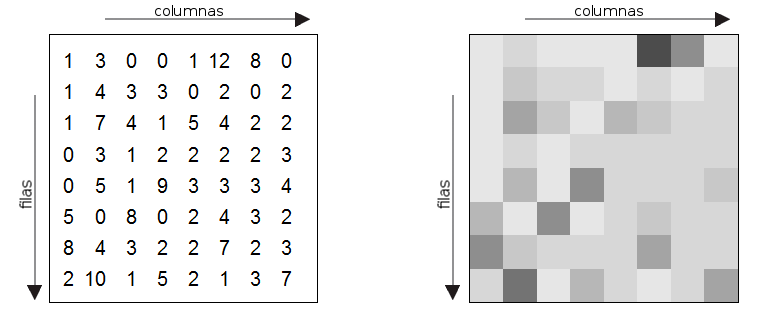
\includegraphics[width=0.9\textwidth]{capitulo-2/graphics/representacion-raster.png}
\caption{\label{fig:sig-capa-raster} Comparación entre la definición de una capa ráster y su representación. }
\end{figure}

La resolución y la nitidez del la capa ráster depende del tamaño de la celda
(\figref{fig:sig-raster-resolucion}), donde el tamaño esta asociado a la cantidad de columnas y
filas de la capa ráster. Mientras más filas y columnas cuente una capa ráster, más nítida será la
imagen resultante.


\begin{figure}[!htbp]
    \centering
    \begin{subfigure}[b]{0.4\textwidth}
            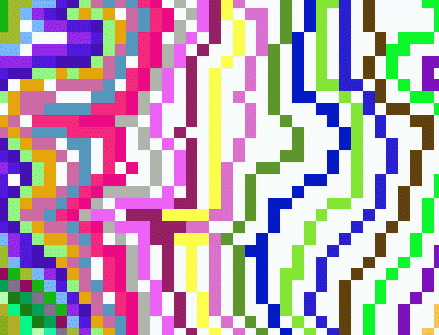
\includegraphics[width=\textwidth]{capitulo-2/graphics/raster-baja-resolucion.png}
            \caption{Tamaño de celda inadecuado, imágen de baja resolución.}
    \end{subfigure}
    ~~~~
    \begin{subfigure}[b]{0.4\textwidth}
            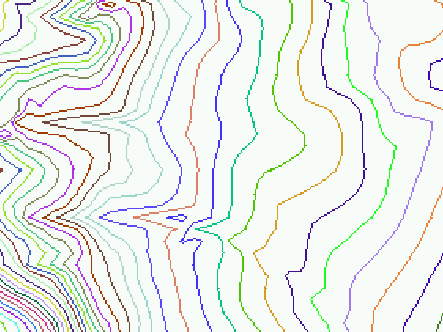
\includegraphics[width=\textwidth]{capitulo-2/graphics/raster-alta-resolucion.png}
            \caption{Tamaño de celda adecuado, imágen de alta resolución.}

    \end{subfigure}
    \caption{\label{fig:sig-raster-resolucion}Curvas de nivel rasterizadas con dos tamaños distintos de celdas y su relación con la resolución de las imagenes resultantes (Tomado de \cite{fAlonsoSig2006}).}
\end{figure}

\subsection{Formato vectorial}
Los datos vectoriales, se caracterizan por la precisión de localización de los elementos
geográficos en el espacio, donde los fenómenos a representar son discretos, con límites bien
definidos. Generalmente se considera que el formato vectorial es más adecuado para la
representación de entidades o variables cualitativas y el formato ráster para representar
superficies\cite{fAlonsoSig2006}.

Los diferentes objetos, vectoriales, se encuentran representados como puntos, lineas o polígonos
\cite{fAlonsoSig2006}. De tal forma que para modelar digitalmente las entidades del mundo real se
utilizan estos tres elementos geométricos.

\begin{figure}[!htbp]
\centering
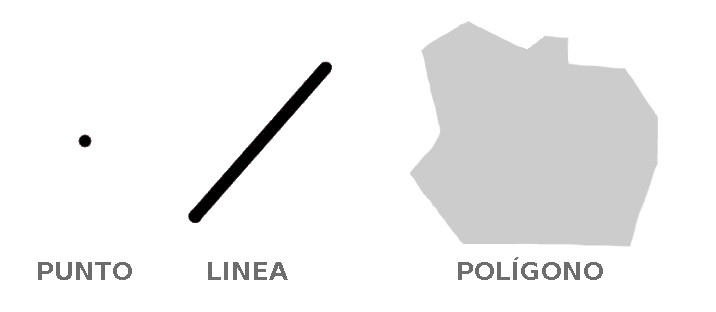
\includegraphics[width=0.8\textwidth]{capitulo-2/graphics/dimensiones-datos.jpg}
\caption{\label{fig:sig-xyz} Elementos geométricos utilizados para modelar digitalmente las entidades en un SIG.}
\end{figure}

\begin{itemize}
    \item \textit{Puntos} : se utilizan para representar las entidades geográficas que pueden ser
    descritas como un fenómeno puntual. Estos transmiten la menor cantidad de información y su representación es la más simple.

    \item \textit{Líneas o polilíneas} : las líneas unidimensionales o polilíneas son usadas para
    representar elementos con rasgos lineales como ríos, caminos, ferrocarriles, rastros, líneas
    topográficas o curvas de nivel.

    \item \textit{Polígonos} : se utilizan para representar elementos geográficos que cubren un
    área particular de la superficie de la tierra. Los polígonos transmiten mayor cantidad de
    información y en ellos se pueden medir el perímetro y el área.
\end{itemize}

\subsection{Ventajas y desventajas de los formatos ráster y vectorial}

El debate acerca de la conveniencia de uno u otro modelo debe basarse en el tipo de estudio o
enfoque que se quiera hacer, pero también del software y fuentes de datos disponibles
\cite{fAlonsoSig2006}.

El formato ráster se considera el más adecuado para representar eficientemente las superficies.
Estas solo pueden representarse vectorialmente mediante modelos híbridos que no resultan adecuados
para la realización de posteriores análisis ya que todas las operaciones que permite el modelo
ráster resultan más lentas con el modelo vectorial \cite{fAlonsoSig2006}. Tradicionalmente se ha
considerado que para la representación de los objetos resulta más eficiente la utilización de un
formato vectorial ya que la estructura de los datos es compacta y almacena los datos sólo de los
elementos digitalizados por lo que requiere menos memoria para su almacenamiento y tratamiento
\cite{fAlonsoSig2006}. Los gráficos vectoriales, se caracterizan por no perder la definición a
media que se aumenta la escala para la visualización.

\begin{figure}[!htbp]
    \centering
    \begin{subfigure}[b]{0.4\textwidth}
            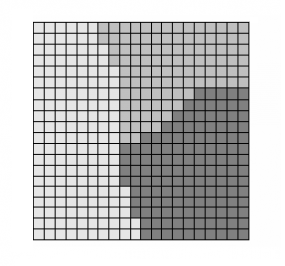
\includegraphics[width=\textwidth]{capitulo-2/graphics/formato-raster.png}
            \caption{Formato ráster.}
    \end{subfigure}
    ~~~~
    \begin{subfigure}[b]{0.4\textwidth}
            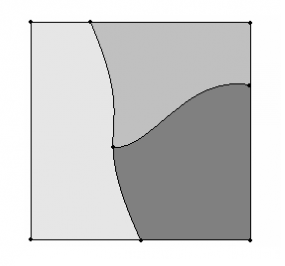
\includegraphics[width=\textwidth]{capitulo-2/graphics/formato-vectorial.png}
            \caption{Formato vectorial.}

    \end{subfigure}
    \caption{\label{fig:sig-raster-vs-vectorial} Representación de una misma superficie, mediante los formatos ráster y vectorial, en un SIG.}
\end{figure}

En general las ventajas del modelo ráster radican en, su simplicidad y la velocidad de ejecución de
los operadores lo que lo convierte en el modelo a utilizar para la representación de modelos
digitales de terreno o imágenes satelitales. Por otro lado, entre sus desventajas podemos
mencionar su inexactitud que depende de la resolución y el tamaño de las celdas, además podemos
mencionar que se requiere una gran cantidad de espacio para el almacenamiento aunque este problema
puede compensarse mediante diversos sistemas de compresión.

Hoy en día se pueden codificar las formas en un modelo vectorial y los procesos con un modelo
ráster, para ello se requieren herramientas eficaces de paso de un formato al otro. Resulta
sencillo, finalmente, la visualización simultánea de datos en los dos formatos gracias a la
capacidad gráfica actual\cite{fAlonsoSig2006}.

%* Análisis espacial con SIG
\section{Análisis espacial en un SIG}
\label{sec:cap2-analisis-espacial-sig}

Un SIG puede reconocer y analizar las relaciones espaciales que existen en la información geográfica almacenada.
Estas relaciones topológicas permiten realizar modelizaciones y análisis espaciales complejos. Así, por ejemplo, 
el SIG puede discernir la parcela o parcelas catastrales que son atravesadas por una línea de alta tensión, o bien
saber qué agrupación de líneas forman una determinada carretera.

En suma podemos decir que en el ámbito de los sistemas de información geográfica se entiende como topología a las 
relaciones espaciales entre los diferentes elementos gráficos (topología de nodo/punto, topología de red/arco/línea, 
topología de polígono) y su posición en el mapa (proximidad, inclusión, conectividad y vecindad). Estas relaciones, 
que para el ser humano pueden ser obvias a simple vista, el software las debe establecer mediante un lenguaje y unas
reglas de geometría matemática.

Para llevar a cabo análisis en los que es necesario que exista consistencia topológica de los elementos de la base de 
datos suele ser necesario realizar previamente una validación y corrección topológica de la información gráfica. 
Para ello existen herramientas en los SIG que facilitan la rectificación de errores comunes de manera automática o 
semiautomática.

La geoestadística analiza patrones espaciales con el fin de conseguir predicciones a partir de datos espaciales concretos.
Es una forma de ver las propiedades estadísticas de los datos espaciales. A diferencia de las aplicaciones estadísticas 
comunes, en la geoestadística se emplea el uso de la teoría de grafos y de matrices algebraicas para reducir el número de 
parámetros en los datos. Tras ello, el análisis de los datos asociados a entidad geográfica se llevaría a cabo en segundo 
lugar.

Cuando se miden los fenómenos, los métodos de observación dictan la exactitud de cualquier análisis posterior. Debido a 
la naturaleza de los datos (por ejemplo, los patrones de tráfico en un entorno urbano, las pautas meteorológicas en el 
océano, etc.), grado de precisión constante o dinámico se pierde siempre en la medición. Esta pérdida de precisión se 
determina a partir de la escala y la distribución de los datos recogidos. Los SIG disponen de herramientas que ayudan a 
realizar estos análisis, destacando la generación de modelos de interpolación espacial.


%* Métodos de interpolación
\section{Métodos de interpolación}
\label{sec:cap2-metodos-interpolacion}

La interpolación espacial, consiste en la utilización de puntos con valores conocidos, también denominados puntos
de control, para estimar una variable en lugares donde se desconoce; también se considera una forma de transformar
información puntual en información de superficie, con el objetivo de combinarla con otros datos para facilitar el
análisis y la modelado espacial.

Todos los métodos de interpolación se basan en la presunción lógica de que cuanto más cercanos están dos puntos
sobre la superficie terrestre, los valores de cualquier variable cuantitativa que midamos en ellos serán más
parecidos, para expresarlo más técnicamente, las variables espaciales muestran autocorrelación espacial \cite{fAlonsoSig2006}.

El resultado de la interpolación espacial depende de un algoritmo computacional o una ecuación matemática en la
cual se emplean los datos de los puntos de control\cite{NINO2011}.


\subsection {Red de Triángulos Irregulares (TIN)}
Las Redes Irregulares de Triángulos (TIN por sus siglas en ingles Triangulated Irregular Network), se generan a
partir de valores puntuales tratando de conseguir triángulos que maximicen la relación área/perímetro, el conjunto
de todos los triángulos forma un objeto geométrico denominado conjunto convexo\cite{fAlonsoSig2006}. Son
ampliamente utilizados como método para la representación de modelos de elevaciones, ya que producen resultados
visualmente muy buenos, sin embargo a la hora de realizar la integración con la información raster restante, se
necesita interpolar una capa raster a partir de los triángulos.

Según \cite{cPachecoMDE2003} TIN utiliza los puntos de entrada para construir una red de triángulos según el
criterio de Delauny: en cada triángulo, el círculo que pasa a través de los tres vértices no encierra ningún otro
punto de entrada (el criterio de Delauny genera, tanto como le es posible, triángulos pequeños y equiláteros y es
ley ser utilizado para crear objetos TIN). Luego, el proceso ajusta una superficie plana a cada triángulo, de
manera tal que el total de la superficie está modelada como una colección de facetas trianguladas planas.


\begin{figure}
\centering
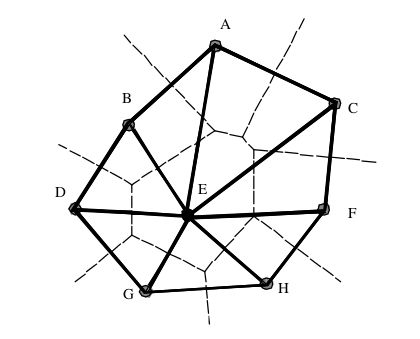
\includegraphics[width=0.4\textwidth]{capitulo-2/graphics/TIN-cPachecoMDE2003.png}
\caption{\label{fig:sig-tin}Red de Triángulos Irregulares (TIN) (Tomado de \cite{cPachecoMDE2003}).}
\end{figure}


\subsection{Ponderación de la inversa de la distancia (IDW)}
Estima los puntos del modelo realizando una asignación de pesos a los datos del entorno en función inversa a la
distancia que los separa del punto en cuestión. De esta forma, se acepta que los puntos más próximos al centroide
intervienen de manera más relevante en la obtención del valor definitivo de Z para ese punto.

La elección del exponente de ponderación(p) determina la contribución de los puntos circundantes al punto 
problema, cuanto mayor es p, más contribuyen los puntos próximos. Es necesario contar con muchos puntos para la
interpolación.

La forma general de encontrar un valor interpolado $u$ en un punto $x$ basado en muestras $u_i = u (x_i)$ para 
$i = 0,1, ..., N$ utilizando IDW es una función de interpolación:

\begin{equation}\label{eq:interpolacion-idw}
 u(x) = \sum_{i=1}^{N} \frac{w_i(X)}{\sum_{j=1}^{N} w_j(X)}
\end{equation}

donde 

\begin{equation} 
w_i(X) =  \frac{1}{d(X, X_i)^p} 
\end{equation}

\subsection{Kriging}
El Kriging es un método geoestadístico de interpolación espacial de carácter global, exacto y estocástico. La 
idea básica de este método corresponde a la noción de dependencia espacial, según la cual las muestras cercanas
tienen mayor similitud entre sí que las más apartadas\cite{NINO2011}.

Se presenta con un método de interpolación con una expresión general similar a la anterior (IDW). La diferencia
básica es que asume que la altitud puede definirse como una variable regionalizada. Supone que la variación
espacial de la variable a representar puede ser explicada al menos parcialmente mediante funciones de correlación
espacial(la variación espacial de los valores de z puede deducirse de los valores circundantes de acuerdo con unas
funciones homogéneas en toda el área).

%* Aplicaciones de SIG y análisis epidemiológicos
\section{Aplicaciones y análisis epidemiologico}
\label{sec:cap2-aplicaciones-analisis-epidemiologico}

Con el correr del tiempo su el potencial ha incrementado rápidamente, desde su concepción en los años setenta,
actualmente las áreas en las que se aplica se ha diversificado, entre las más resaltantes podemos nombrar:
biología, energía e infraestructura, planificación urbana y regional, monitoreo ambiental y geografía física,
transportación y logística. Entre las aplicaciones más usuales destacan las del campo científico, gestión 
y empresarial. 

Las autoridades sanitarias, en sus tareas de vigilancia en Salud Pública, tienen en los GIS una 
herramienta fundamental para conocer cómo se extiende una enfermedad, estudiar su posible relación 
con un potencial foco de riesgo, o localizar un brote epidémico\cite{vgomesAegis2001}. 

Los análisis más utilizados por las entidades sanitarias son la cartografía de enfermedades, cuyo fin es
representar la distribución espacial de la enfermedad,  y el análisis de focos de riesgo, que establece 
bandas alrededor de un punto o una zona geográfica representando una potencial fuente contaminante para 
comparar el riesgo de una enfermedad en cada una de esas bandas. La información necesaria para realizar 
este tipo de estudios proviene de muy diversas fuentes: registros de mortalidad, hospitales, facultativos, 
bases de datos oficiales, observatorios medioambientales o meteorológicos, proyectos específicos. Por 
tanto, es muy importante recopilar y tratar de forma unificada toda esta información para facilitar su 
acceso y análisis.

Los SIG son capaces de simplificar grandes tareas como la localización de eventos en espacio y tiempo, 
el monitoreo de eventos de salud y el comportamiento de factores de riesgo en un período de tiempo dado, la
identificación de áreas geográficas y grupos de población con grandes necesidades de salud y contribuye a la
solución de tales necesidades mediante el análisis de múltiples variables y la evaluación del impacto de
intervenciones en salud\cite{iMolinaSigEpidemiologia}.


%\chapter{Aedes aegypti, principal transmisor del dengue}
%* Historia de la enfermedad

\section{El virus del dengue}

\subsection{Introducción}
El dengue es una enfermedad infecciosa causada por el virus del dengue transmitida por el mosquito Aedes Aegypti que puede ser mortal. La probabilidad de mortalidad puede verse reducida en 0.001 en el caso de ser tratado a tiempo.\\

Afecta a paises en regiones tropicales con climas calidos principalmente en zonas urbanas. La enfermedad causa sindromes gripales como fiebre, tos, dolor de cabeza, resfrio, dolor de garganta y musculos. La lucha contra el flagelo de la enfermedad depende de forma exclusiva de las medidas para controlar el vector que transmite la enfermedad, el mosquito Aedes Aegypti\\

El dengue hemorragico es mas comun en pacientes que ya han padecido la enfermedad con anterioridad. Existen diferentes serotipos de la enfermedad y en el caso de haber padecido un serotipo primario existe la posibilidad que ante un nuevo contagio se desarrolle otro serotipo lo cual derive en el padecimiento de caso de dengue hemorragico

\subsection{Epidemiología}

Durante la decada 2000 se ha visto un notable crecimiento de afectados de la enfermedad en la zona de america latina en paises como Paraguay, Brasil, Venezuela Peru. Principalmente en nuestro pais, Paraguay, existen epidemias  de distintos grados de gravedad en cada temporada de verano. Estas epidemias son ocasionadas principalmente por la falta de medidas de prevencion y control contra el mosquito transmisor Aedes Aegypti.\\

Si bien es cierto que se realizan campañas contra la enfermedad, los recorridos de fumigacion y limpieza terminan siendo obsoletos ante el no despertar ciudadano frente a la enfermedad. La existencia de grandes cantidades de patios baldios y terrenos sucios en zonas urbanas dificulta la eliminacion del agente transmisor y como consecuencia la enfermedad prevalece y se propaga.\\

La cantidad de afectados por la enfermedad en los ultimos años en todo Paraguay son:
\begin{itemize}
\item 13.766 casos en el año 2010
\item 42.945 casos en el año 2011
\item 2.347 casos en el año 2012
\item 130.155 casos en el año 2013\\
\end{itemize}

El aumento de la población del vector en zonas urbanas del pais, la masiva presencia del virus dengue en los países vecinos, la no colaboración de la poblacion para la eliminacion de criaderos de mosquitos de Aedes aegypti, además de la gran circulación de la poblacion en entre zonas habitadas son alguno de los factores que permiten que la enfermedad siga provocando olas de alerta y riesgo. A estos factores hay qye sumar el factor de la temperatura de nuestro país que es ideal para el desarrollo del agente transmisor.\\


Uno de los objetivos criticos es proveer un sistema de informacion que permita accionar preventivo en zonas de posibles focos de la enfermedad. Cada año en las ultimas 2 decadas se revive la misma situacion, hospitales abarrotados, escases de medicos y medicamentos, situacion de alerta, colapso social ante la epidemia.\\

\subsection{Distribucion Geografica}

El dengue es una enfermedad presente en todo el territorio del Paraguay con fuerte presencia desde hace una decada. Pero la distribucion de la enfermedad no es homogenea sino que se mapea a nivel macro a la distribucion de la poblacion. De ahí que el departamento central es uno de los departamentos con mayor indice de infestación de la enfermedad. En la figura 1 se obserba el resumen de los primeros meses del 2014. Departamentos clasificados segun sean zonas endemicas o no. Los departamentos con mayor densidad poblacional y movimiento de personas son siempre zonas endemicas.\\

Las zonas más afectadas en nuestro país son los departamentos de Central, Amambay e Itapúa. Seguidos de Coordillera, Paraguari y Alto Parana. Otras zonas y departamentos también presentan casos de la enfermedad solo que no son consideradas zonas endemicas o de riesgo. Esta distribución que denota las zonas de mayor riesgo se repite en cada época de flagelo de la enfermedad.\\

A nivel intrinseco en los objetivos de este trabajo está realizar resumenes en mapas similares a los que se muestran en las figuras 1, 2 y 3 pero conteniendo informacion a priori sobre la enfermedad. No señalar las zonas endemicas o no endemicas sino señalar las posibles zonas endémicas o no endémicas según información recolectada sobre la distribución larvaria. Esto permitiría realizar planes de control y prevención de la enfermedad.\\

\begin{figure}
\centering
%\includegraphics[width=0.8\textwidth]{Diapositiva03.JPG}
\caption{\label{fig:mapa1}Zonas endemicas en todo el pais. Anho 2014}
\end{figure}

\begin{figure}
\centering
%\includegraphics[width=0.8\textwidth]{Diapositiva04.JPG}
\caption{\label{fig:mapa2}Mapa de riesgo de la semana epidermiologica 05. Anho 2013 }
\end{figure}

\begin{figure}
\centering
%\includegraphics[width=0.8\textwidth]{Diapositiva05.JPG}
\caption{\label{fig:mapa3}Mapa del area metropolitana de Asuncion.}
\end{figure}

\subsection{Salud publica}
Cada año el ministerio de salud pública y bienestar social (MSPyBS) en conjunto con otras organizaciones estatales y privadas realiza un plan de de acción en contra de la enfermedad. Un documento detallado presenta el proyecto y los responsables de llevarlo a cabo. El problema de los planes de acción es la dependencia del accionar ciudadano.
Del documento Dengue Plan 12 11 13 del MSPyBS se menciona los objetivos del plan de acción: \\

\textit{"...Los objetivos específicos para cada pilar son los siguientes:\\
\begin{enumerate}
\item Coordinación y Planificación: Fomentar el trabajo intersectorial, el monitoreo y la difusión del plan de acción
\item Vigilancia Entomológica: Vigilar, informar y alertar sobre riesgos ambientales
\item Control Vectorial: Disminuir la población de mosquitos
\item Vigilancia Laboratorial: Garantizar la representatividad de la vigilancia
\item Laboratorio de apoyo en Servicios: Garantizar el acceso a pruebas laboratoriales de diagnóstico
\item Vigilancia Epidemiológica: Aumentar la sensibilidad y oportunidad de la vigilancia
\item Componente Ambiental: Promover intervenciones sobre determinantes de la presencia del mosquito
\item Promoción y Participación Social: Fomentar la movilización social en acciones de control y prevención
\item Comunicación: Informar a la población sobre la problemática del dengue
\item Atención Integral: Asegurar la atención adecuada y oportuna a las personas con síndrome febril agudo con sospecha de dengue..."
\end{enumerate}}

Se concluye de los objetivos la dependencia del accionar de la población. Sin el apoyo de la ciudadanía no es posible controlar el vector ni realizar una vigilancia efectiva . La participación ciudadana tiene que empezar desde el conocimiento de la enfermedad y del vector transmisor. A eso debe sumarse la predisposición para realizar la limpieza del hogar/es propios mediante la eliminación de recipientes que acumulen agua principalmente. El problema es la enorme cantidad de patios baldíos y terrenos desabitados que luego de lluvias terminan siendo sitios propensos para alojar al mosquito.\\


La propuesta realizada en este trabajo tambíén requiere de la participación de la ciudadanía, pero desde un punto de vista distinto ya que el plan de acción será aplicado a las zonas de alto índice de población larval en primer lugar, permitiendo optimizar recursos y fuerza. Requerir de la acción ciudadana luego de que se presenten casos de la enfermedad se torna imposible, el estado de alerta desata preocupación y poco interés en luchar contra la enfermedad. La población en caso de riesgo busca refugiarse del la ola de la enfermedad y aunque existe colaboración para realizar un control sobre el vector el hecho de que ya exista afectados impide lograr una lucha eficiente.

\section{Aedes Aegypti. Mosquito transmisor del dengue}
El Aedes Aegypti  es el principal transmisor de la enfermedad del dengue. Es un mosquito que tiene como principales caracteristicas su contextura oscura y pequeña y sus manchas blancas en las extremidades. Mide apróximadamente 5mm. Al igual, evidentemente, que la enfermedad del dengue el mosquito se encuentra en zonas urbanas de regiones y paises tropicales.\\

Se estima que el mosquito causa mas de 50 millones de infecciones y mas de 26.000 muertes por año
Se recomiendan como metodo preventivo la utilizacion de repelentes que contengan DEET ya que son considerados como el mejor repelente contra el mosquito\\

\subsection{Biología}

El ciclo de vida del Aedes Aegypti es comun como otros mosquitos de especies similares. Basicamente consta de 4 estados:\\
\begin{itemize}
\item Huevo
\item Larva
\item Pupa
\item Adulto\\
\end{itemize}

Los huevos son depositados en las paredes de los recipientes por encima del nivel del agua. Los mismos son resitentes a temporadas de sequías largas. El contacto del agua con los huevos el paso a la siguiente etapa del mostiquito.\\

Los huevos eclosionan y pasan al estado de larvas. Las larvas son individuos móviles que se alimentan de residuos orgánicos encontrados en las paredes y fondos de los recipientes que los contienen. El paso a la siguiente etapa depende de la cantidad de alimentos, la temperatura y la densidad de larvas en el recipiente. Si se dan las condiciones se produce la metamorfosis y pasa al estado de pupa.\\

Las pupas no se alimentan, flotan en la superficie hasta alcanzar el estado adulto en aproximadamente 2 a 4 dias. El tiempo total de huevo a adulto es entre 7 a 14 dias. El tiempo es variable segun la duracion de cada cambio de estado.\\

El adulto se alimenta del nectar y aceites de plantas, pero la hembra del aedes aegipty necesita alimentarse de sangre para la formacion de los huevos y lo hace atravez de cualquier vertebrado teniendo preferencia por el humano.\\

Sus hábitos alimenticios pueden describirse por franjas horarias ya que se alimentan al amanecer y al atardecer. Buscan lugares oscuros de donde emerger y atacan a la victima en la piel cualquier parte del cuerpo  descubierta. Son muy habituales las picaduras en las manos, brazos, cuello, piernas. El contagio se produce cuando el mosquito hembra se alimenta de sangre humana infectada con el virus y luego pica a otro humano. No puede transmitirse de forma directa entre humano y humano\\

Su habitat para reproduccion y ovipostura son los lugares con agua estancada preferentemente limpia, lugares oscuros y quietos tales como latas, botellas vacías, neumáticos usados, baldes, etc.\\

\subsection{Cambios Climáticos}

Uno de los aspectos más importantes del mosquito Aedes Aegypti es su dependencia a la temperatura. Un país con temperatura tropical (promedio 25º C.) es un país ideal para la supervivencia del Aedes Aegypti no así un país con extremo calor o un clima más frío. Cada etapa de su desarrollo está ligado a condiciones climáticas; no solo temperatura sino también, lluvias y humedad. La lluvia permite que el agua se acumule en distintos recipientes; barriles, llantas y cubiertas, planteras, canaletas, etc. Se realizaron varios estudios analizando la influencia de la temperatura en el desarrollo del mosquito Aedes Aegypti. De los resultados de las pruebas se pueden obtener datos como el promedio de días en el que se pasa del estado larva a pupa ver Cuadro 1.\\

Esta información es muy valiosa en el estudio del mosquito ya que con el pronóstico del tiempo uno puede estimar el tiempo de desarrollo del Aedes Aegypti y determinar el crecimiento de la población actual (por ej. En 15 días aumentará la población actual del Aedes Aegypti en un 20\% dada las condiciones del clima previsto en esta zona)

\subsection{Ciclo gonadotrófico}
Después de cada alimentación se desarrolla un lote de huevos. Si la hembra completa su alimentación sanguínea (2-3 mg) desarrollará y pondrá 100-200 huevos, el intervalo dura de dos a tres días. La hembra grávida buscará recipientes oscuros o sombreados para depositar sus huevos, prefiriendo aguas limpias y claras.\\

\subsection{Rango de vuelo}
La hembra no sobrepasa los 50-100 m durante su vida (puede permanecer en la misma casa donde emergió). Si no hay recipientes, una hembra grávida puede volar tres kilómetros para poner sus huevos. Los machos se dispersan menos que las hembras.\\

\subsection{Conducta de reposo}
Descansan en lugares sombreados como alcobas, baños, patios o cocinas. Se les captura sobre ropas colgadas, debajo de muebles, toallas, cortinas y mosquiteros.\\

\subsection{Longevidad}
Los adultos pueden permanecer vivos en el laboratorio durante meses y en la naturaleza pocas semanas. Con una mortalidad diaria de 10\%, la mitad de los mosquitos morirán durante la primera semana y 95\% en el primer mes.\\


\begin{table}
\centering
\begin{tabular}{l|r}
Temperatura & Tiempo en estado larval y pupa \\\hline
13 & 0 \\
15-20 & 10 a 17.4 \\
20-25 & 9 a 13 \\
25-36 & 5 a 7 \\
36+ & 0
\end{tabular}
\caption{\label{tab:widgets}Tiempo promedio de duración en días del estado larval y pupa a diferentes temperaturas.}
\end{table}

%* Dengue en Paraguay
%* Distribución geográfica
%* Salud pública

\subsection{Epidemiología}

Durante la década 2000 se ha visto un notable crecimiento de afectados de la enfermedad en la zona de América latina en países como Paraguay, Brasil, Venezuela Perú. Principalmente en nuestro país, Paraguay, existen epidemias  de distintos grados de gravedad en cada temporada de verano. Estas epidemias son ocasionadas principalmente por la falta de medidas de prevención y control contra el mosquito transmisor Aedes Aegypti.\\

Si bien es cierto que se realizan campañas contra la enfermedad, los recorridos de fumigacion y limpieza terminan siendo obsoletos ante el no despertar ciudadano frente a la enfermedad. La existencia de grandes cantidades de patios baldíos y terrenos sucios en zonas urbanas dificulta la eliminacion del agente transmisor y como consecuencia la enfermedad prevalece y se propaga.\\

La cantidad de afectados por la enfermedad en los ultimos años en todo Paraguay son:
\begin{itemize}
\item 13.766 casos en el año 2010
\item 42.945 casos en el año 2011
\item 2.347 casos en el año 2012
\item 130.155 casos en el año 2013\\
\end{itemize}

El aumento de la población del vector en zonas urbanas del país, la masiva presencia del virus dengue en los países vecinos, la no colaboración de la poblacion para la eliminación de criaderos de mosquitos de Aedes aegypti, además de la gran circulación de la poblacion en entre zonas habitadas son alguno de los factores que permiten que la enfermedad siga provocando olas de alerta y riesgo. A estos factores hay qye sumar el factor de la temperatura de nuestro país que es ideal para el desarrollo del agente transmisor.\\


Uno de los objetivos criticos es proveer un sistema de informacion que permita accionar preventivo en zonas de posibles focos de la enfermedad. Cada año en las ultimas 2 decadas se revive la misma situacion, hospitales abarrotados, escases de medicos y medicamentos, situacion de alerta, colapso social ante la epidemia.\\

\subsection{Distribucion Geografica}

El dengue es una enfermedad presente en todo el territorio del Paraguay con fuerte presencia desde hace una decada. Pero la distribucion de la enfermedad no es homogenea sino que se mapea a nivel macro a la distribucion de la poblacion. De ahí que el departamento central es uno de los departamentos con mayor indice de infestación de la enfermedad. En la figura 1 se obserba el resumen de los primeros meses del 2014. Departamentos clasificados segun sean zonas endemicas o no. Los departamentos con mayor densidad poblacional y movimiento de personas son siempre zonas endemicas.\\

Las zonas más afectadas en nuestro país son los departamentos de Central, Amambay e Itapúa. Seguidos de Coordillera, Paraguari y Alto Parana. Otras zonas y departamentos también presentan casos de la enfermedad solo que no son consideradas zonas endemicas o de riesgo. Esta distribución que denota las zonas de mayor riesgo se repite en cada época de flagelo de la enfermedad.\\

A nivel intrinseco en los objetivos de este trabajo está realizar resumenes en mapas similares a los que se muestran en las figuras 1, 2 y 3 pero conteniendo informacion a priori sobre la enfermedad. No señalar las zonas endemicas o no endemicas sino señalar las posibles zonas endémicas o no endémicas según información recolectada sobre la distribución larvaria. Esto permitiría realizar planes de control y prevención de la enfermedad.\\

\begin{figure}
\centering
\includegraphics[width=0.8\textwidth]{./graphics/Diapositiva03.JPG}
\caption{\label{fig:mapa1}Zonas endemicas en todo el pais. Anho 2014}
\end{figure}

\begin{figure}
\centering
\includegraphics[width=0.8\textwidth]{./graphics/Diapositiva04.JPG}
\caption{\label{fig:mapa2}Mapa de riesgo de la semana epidermiologica 05. Anho 2013 }
\end{figure}

\begin{figure}
\centering
\includegraphics[width=0.8\textwidth]{./graphics/Diapositiva05.JPG}
\caption{\label{fig:mapa3}Mapa del area metropolitana de Asuncion.}
\end{figure}

\subsection{Salud publica}
Cada año el ministerio de salud pública y bienestar social (MSPyBS) en conjunto con otras organizaciones estatales y privadas realiza un plan de de acción en contra de la enfermedad. Un documento detallado presenta el proyecto y los responsables de llevarlo a cabo. El problema de los planes de acción es la dependencia del accionar ciudadano.
Del documento Dengue Plan 12 11 13 del MSPyBS se menciona los objetivos del plan de acción: \\

\textit{"...Los objetivos específicos para cada pilar son los siguientes:\\
\begin{enumerate}
\item Coordinación y Planificación: Fomentar el trabajo intersectorial, el monitoreo y la difusión del plan de acción
\item Vigilancia Entomológica: Vigilar, informar y alertar sobre riesgos ambientales
\item Control Vectorial: Disminuir la población de mosquitos
\item Vigilancia Laboratorial: Garantizar la representatividad de la vigilancia
\item Laboratorio de apoyo en Servicios: Garantizar el acceso a pruebas laboratoriales de diagnóstico
\item Vigilancia Epidemiológica: Aumentar la sensibilidad y oportunidad de la vigilancia
\item Componente Ambiental: Promover intervenciones sobre determinantes de la presencia del mosquito
\item Promoción y Participación Social: Fomentar la movilización social en acciones de control y prevención
\item Comunicación: Informar a la población sobre la problemática del dengue
\item Atención Integral: Asegurar la atención adecuada y oportuna a las personas con síndrome febril agudo con sospecha de dengue..."
\end{enumerate}}

Se concluye de los objetivos la dependencia del accionar de la población. Sin el apoyo de la ciudadanía no es posible controlar el vector ni realizar una vigilancia efectiva . La participación ciudadana tiene que empezar desde el conocimiento de la enfermedad y del vector transmisor. A eso debe sumarse la predisposición para realizar la limpieza del hogar/es propios mediante la eliminación de recipientes que acumulen agua principalmente. El problema es la enorme cantidad de patios baldíos y terrenos desabitados que luego de lluvias terminan siendo sitios propensos para alojar al mosquito.\\


La propuesta realizada en este trabajo tambíén requiere de la participación de la ciudadanía, pero desde un punto de vista distinto ya que el plan de acción será aplicado a las zonas de alto índice de población larval en primer lugar, permitiendo optimizar recursos y fuerza. Requerir de la acción ciudadana luego de que se presenten casos de la enfermedad se torna imposible, el estado de alerta desata preocupación y poco interés en luchar contra la enfermedad. La población en caso de riesgo busca refugiarse del la ola de la enfermedad y aunque existe colaboración para realizar un control sobre el vector el hecho de que ya exista afectados impide lograr una lucha eficiente.

%* Características biológicas de Aedes aegypti
%* Factores ecológicos y productividad de Aedes aegypti

\section{Ciclo biológico del Aedes aegypti}
\label{sec:caracteristicas-biologicas}
De todas las especies de mosquitos conocidos, con importancia en salud pública, la Aedes aegypti,
es considerada la más peligrosa por tener la capacidad de transmitir el mayor número de enfermedades arbovirales\footnote{Las infecciones arbovirales son los virus que se transmiten por
los mosquitos. \textit{Arbo} es una abreviatura que significa transmitida por los artrópodos, los
cuales son insectos.}, al hombre \cite{ThironIzcazaJ2003}.

Los sitios de cría del Aedes aegypti son fundamentalmente artificiales: urbanos (en baldíos,
cementerios, desarmaderos, basurales) o domésticos (neumáticos, floreros, botellas, bebederos de
animales, latas abiertas o contenedores de cualquier tipo, cisternas, vasijas, tinajas, todo tipo
de recipientes en desuso, aun pequeños, prácticamente de cualquier objeto que retenga agua)
\cite{world2009dengue, directricesDetvArg}.

\begin{figure}[!htbp]
\centering
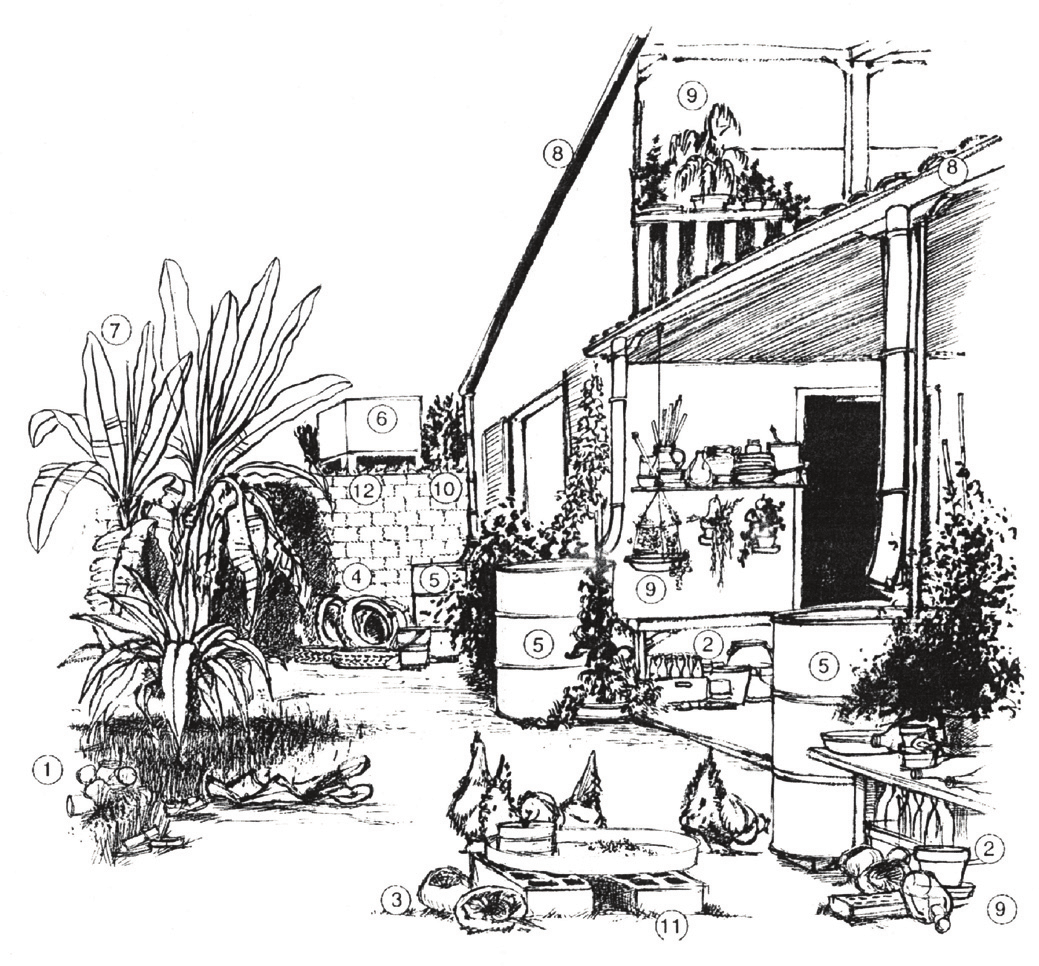
\includegraphics[width=0.8\textwidth]{capitulo-3/graphics/criaderos-domicilio.png}
\caption{\label{fig:cap3-larvitrampas} Ejemplo de los posibles lugares de cría del mosquito Aedes
aegypti, en los alrededores de la casa (Tomado de \cite{manualControlArg2009}).}
\end{figure}


Prefieren agua limpia, con bajo tenor orgánico y de sales disueltas. La puesta de huevos la
realizan en la superficie del recipiente. Algunos recipientes le son más atractivos que otros, en
especial los de color oscuro, de boca ancha, que están al nivel del suelo y se encuentran en la
sombra \cite{ThironIzcazaJ2003}.

Su ciclo de vida manifiesta una metamorfosis completa, es decir que las formas inmaduras salidas
del huevo son completamente diferentes al adulto, las primeras son de vida acuática, las segundas
de vida aérea \cite{directricesDetvArg}, donde su desarrollo se encuentra dividido en cuatro
etapas, huevo, larva, pupa y adulto \cite{web-site:gMonteroBiologia}
(\figref{fig:cap3-ciclo-de-vida}).

\begin{figure}[!htbp]
\centering
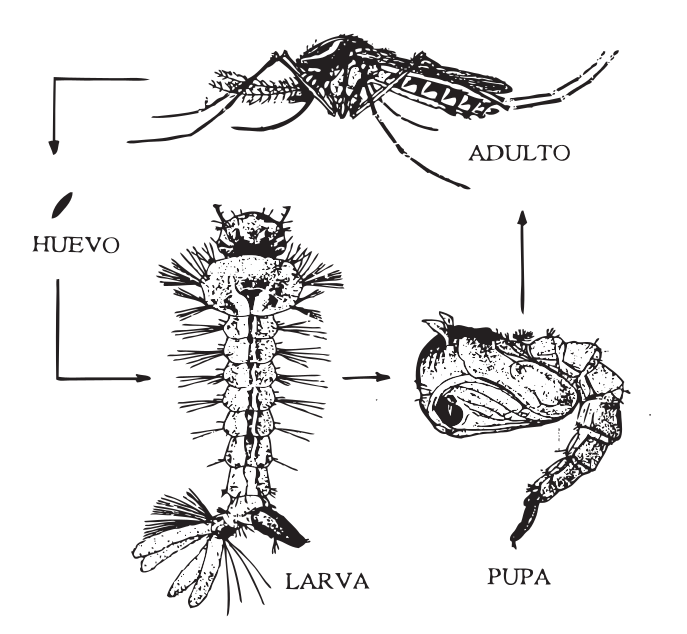
\includegraphics[width=0.7\textwidth]{capitulo-3/graphics/ciclo-de-vida.png}
\caption{\label{fig:cap3-ciclo-de-vida} Ciclo de vida del Aedes aegypti (Tomado de
\cite{directricesDetvArg}).}
\end{figure}

\subsection{Huevo}
\label{subsec:ciclo-biologico-huevo}
Los huevos miden aproximadamente un milímetro de longitud, son depositados uno a uno al ras del agua quedando adheridos a las paredes del recipiente \cite{ThironIzcazaJ2003}. Cada vez que sube el
nivel del agua en el recipiente eclosiona un grupo de huevos, de este modo, se aseguran una
eclosión escalonada que permite la supervivencia aún en condiciones desfavorables
\cite{directricesDetvArg}.

\begin{figure}[!htbp]
\centering
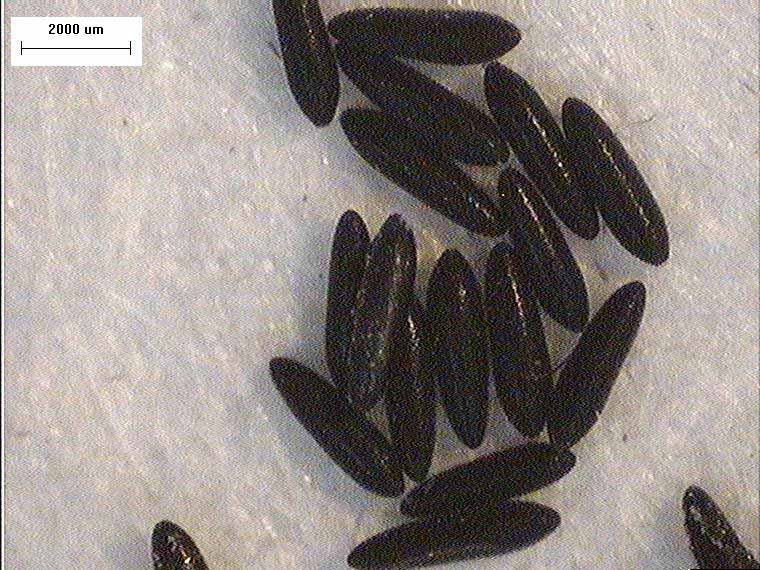
\includegraphics[width=0.5\textwidth]{capitulo-3/graphics/huevos.png}
\caption{\label{fig:cap3-huevos} Huevos del mosquito Aedes aegypti (Tomado de
\cite{sivanathan2006ecology}).}
\end{figure}

Al momento de la postura son de coloración blanca, casi transparentes, en contacto con el aire van
adoptando la coloración oscura característica \cite{directricesDetvArg} (\figref{fig:cap3-huevos}).
La fecundación ocurre al momento de la postura del huevo, en donde el desarrollo embrionario
transcurre en alrededor de 48 horas si el ambiente es húmedo y cálido, si la temperatura es baja
se prolonga hasta por cinco días \cite{ThironIzcazaJ2003}. Los huevos son formas de resistencia que
pueden sobrevivir durante muchos meses en clima adverso hasta que las condiciones ambientales
favorezcan su eclosión \cite{directricesDetvArg}.

\subsection{Larva}
\label{subsec:ciclo-biologico-larva}
Los huevos eclosionan dando lugar a formas larvarias, acuáticas, nadadoras, de respiración aérea
\cite{directricesDetvArg} y es el período de mayor alimentación y crecimiento
\cite{web-site:gMonteroBiologia}. Pasan la mayor parte del tiempo alimentándose del material
orgánico sumergido o acumulado en las paredes y el fondo del recipiente
\cite{web-site:gMonteroBiologia, directricesDetvArg}.

Las larvas que emergen inician un ciclo de 4 estadios larvales \cite{web-site:gMonteroBiologia},
donde, estos estadios definen su período de crecimiento y desarrollo \cite{ThironIzcazaJ2003}. El
primer estadio larval es la forma que emerge del huevo, con una duración de uno a dos días. Este
periodo esta dedicado a la alimentación y el crecimiento, posteriormente ocurre la muda y surge el
segundo estadio \cite{ThironIzcazaJ2003}. En el segundo estadio, la cápsula cefálica y el sifón
son blandos y transparentes, al extenderse permite el subsecuente desarrollo, se endurecen y
oscurecen \cite{ThironIzcazaJ2003}. Después del segundo estadio, la cápsula cefálica y el sifón no
cambian de tamaño, el tórax y el abdomen crecen considerablemente durante cada fase
\cite{ThironIzcazaJ2003}.

\begin{figure}[!htbp]
\centering
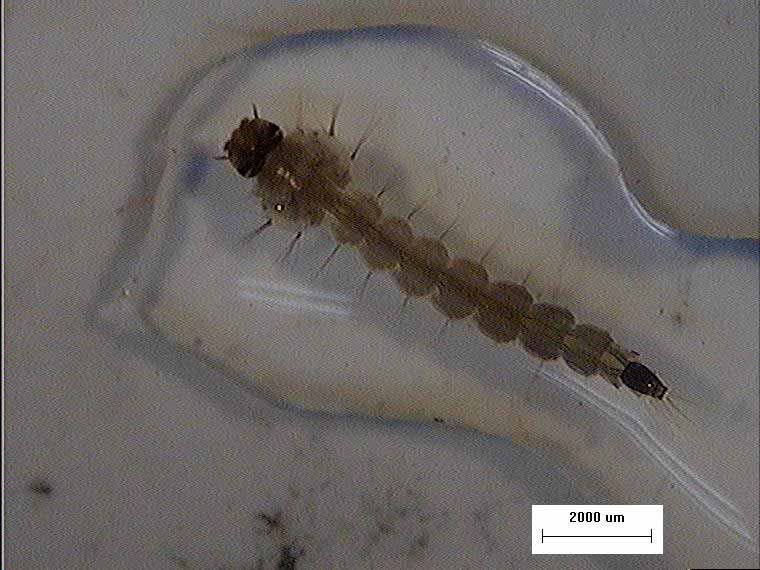
\includegraphics[width=0.5\textwidth]{capitulo-3/graphics/larva.png}
\caption{\label{fig:cap3-larvas} Larva del mosquito Aedes aegypti (Tomado de
\cite{sivanathan2006ecology}).}
\end{figure}

La duración del desarrollo larval está en función de la temperatura, la disponibilidad de alimento
y la densidad de larvas en el criadero \cite{ThironIzcazaJ2003}. Los primeros tres estadios se
desarrollan rápidamente, mientras que el cuarto toma más tiempo, debido a que aumenta
considerablemente su tamaño y peso \cite{ThironIzcazaJ2003, web-site:gMonteroBiologia},
en condiciones de baja temperatura o escasez de alimento el cuarto estadio puede prolongarse por
varias semanas \cite{ThironIzcazaJ2003}. En condiciones óptimas, el período larval desde la
eclosión hasta la pupación puede ser de cinco días, pero por lo regular ocurre de siete a catorce
días \cite{ThironIzcazaJ2003}.

La mortalidad, más elevada ocurre frecuentemente en los primeros estadios larvales
\cite{ThironIzcazaJ2003}, donde la principal causa es atribuida a la inestablididad de los
criaderos que sirven como habitad.

\subsection{Pupa}
\label{subsec:ciclo-biologico-pupa}
Las pupas, al igual que las larvas, son acuáticas, estas no se alimentan, su función es la
metamorfosis del estadio larval al adulto \cite{ThironIzcazaJ2003}. El período pupal dura de 1
a 3 días en condiciones favorables, con temperaturas entre 28 y 32 \textcelsius
\cite{web-site:gMonteroBiologia}, emergiendo alrededor del 88\% de los adultos en cuestión de 48
horas \cite{ThironIzcazaJ2003}. Las variaciones extremas de temperatura pueden dilatar este período
\cite{web-site:gMonteroBiologia}.

\begin{figure}[!htbp]
\centering
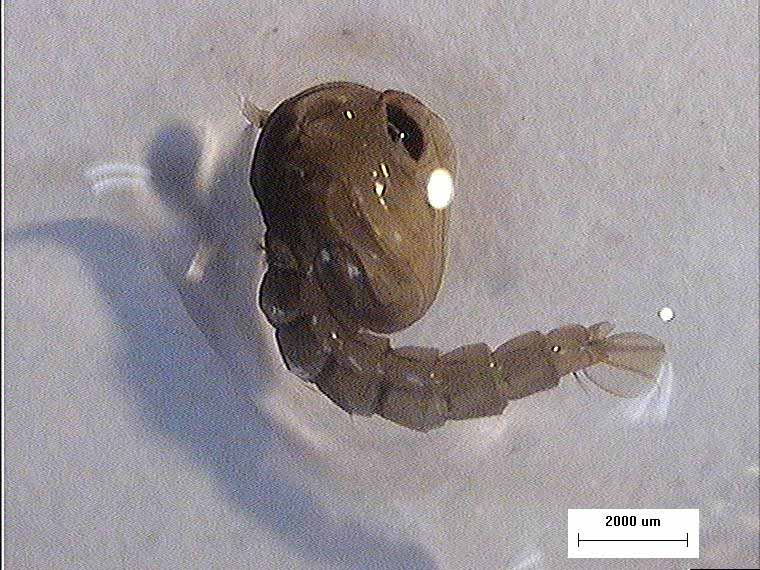
\includegraphics[width=0.5\textwidth]{capitulo-3/graphics/pupa.png}
\caption{\label{fig:cap3-larvas} Larva del mosquito Aedes aegypti (Tomado de
\cite{sivanathan2006ecology}).}
\end{figure}

\subsection{Adulto}
\label{subsec:ciclo-biologico-adulto}
La función más importante del adulto es la reproducción \cite{ThironIzcazaJ2003}. Aproximadamente
la mitad de los adultos emergentes son hembras \cite{otero2006stochastic, manrique1998desarrollo}.
Los adultos recién emergidos permanecen las primeras 24 horas en fase teneral\footnote{Período en
que el insecto adulto está recién salió de la envoltura pupal o piel de ninfa.}, tiempo en que se
efectúa el endurecimiento y oscurecimiento de su cutícula \cite{luevano1993ciclo}. Pueden
permanecer vivos en el laboratorio durante meses y en la naturaleza pocas semanas, con una
mortalidad diaria de 10\%, la mitad de los mosquitos morirán durante la primera semana y 95\% en
el primer mes \cite{ThironIzcazaJ2003}.

\begin{figure}[!htbp]
\centering
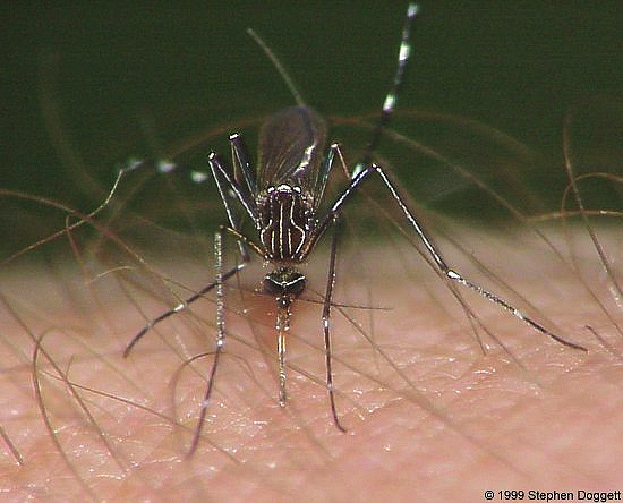
\includegraphics[width=0.5\textwidth]{capitulo-3/graphics/adulto.png}
\caption{\label{fig:cap3-larvas} Adulto del mosquito Aedes aegypti (Tomado de
\cite{directricesDetvArg}).}
\end{figure}

Las partes bucales del macho no están adaptadas para chupar sangre, se alimentan de carbohidratos
de cualquier fuente accesible como frutos o néctar de flores que satisface sus requerimientos
energéticos \cite{ThironIzcazaJ2003}. Las hembras también se alimentan de esta misma fuente como
complemento indispensable, sin embargo necesitan alimentarse de sangre para obtener las proteínas
necesarias para la formación de los huevos \cite{ThironIzcazaJ2003}.

Antes de 24 horas ambos sexos están listos para el apareamiento, alrededor del 58\% de las hembras
nulíparas \footnote{Nulíparas son aquellas hembras jóvenes que no han ovipuesto.} son inseminadas
antes de su primera alimentación sanguínea, un 17\% durante y el 25\% es inseminada entre la
segunda alimentación y la primera oviposición \cite{ThironIzcazaJ2003}. Una inseminación es
suficiente para fecundar todos los huevos que la hembra produzca en toda su vida
\cite{ThironIzcazaJ2003}. El apareamiento, que por lo general se efectúa durante el vuelo, es
debido a que el macho es atraído por el sonido emitido por las alas de la hembra
\cite{ThironIzcazaJ2003}. El patrón diario de alimentación de los mosquitos, varia de acuerdo a
las localidades y subespecies\cite{luevano1993ciclo}.

Los mosquitos tienen la particularidad de volar en sentido contrario a la dirección al viento
\cite{ThironIzcazaJ2003, web-site:speedAnimals} a una velocidad máxima de dos kilómetros por hora
\cite{web-site:speedAnimals,kaufmann2004flight}. Por sus hábitos, es considerado como doméstico
\cite{luevano1993ciclo}, tiende a permanecer en el lugar en donde emergió
\cite{cabezas2005dengue,ThironIzcazaJ2003}, siempre y cuando no exista algún factor que la
perturbe o no disponga de huéspedes, sitios de reposo y de postura  \cite{ThironIzcazaJ2003}. Por
lo general el mosquito no sobrepasa los 50 a 100 metros durante su vida \cite{cabezas2005dengue}.
Los sitios de cría del Aedes aegypti son fundamentalmente artificiales o domésticos
\cite{directricesDetvArg}. En caso de no haber recipientes adecuados, la hembra grávida es capaz
de volar hasta tres kilómetros en busca de este sitio \cite{ThironIzcazaJ2003}.

Es común que después de cada alimentación sanguínea la hembra desarrolle un lote de huevos, la
cantidad de huevos depende de la alimentación que puede variar entre 100 a 200 huevos
\cite{cabezas2005dengue}. El intervalo de tiempo que transcurre entre la alimentación sanguínea y
la postura, denominado ciclo gonotrófico, es de 48 horas en los trópicos bajo condiciones óptimas
de temperatura\cite{ThironIzcazaJ2003}. Dentro de la bionomía de vectores, una fase muy importante
es el ciclo gonotrófico, el cual es un proceso fisiológico que consiste en la digestión de la
comida sanguínea y desarrollo de los ovarios \cite{luevano1993ciclo}.


\section{Aedes aegypti y el cambio climático}
Los cambios temporales y espaciales en la temperatura, precipitaciones y humedad que se prevé que ocurran bajo
diferentes escenarios de cambio climático afectarán la biología y ecología de Ae. aegypti y, en consecuencia, 
los riesgos de transmisión de la enfermedad del dengue\cite{dengueUruguayCap2}.

%Reescribir esta parte%
Los mayores efectos del cambio del clima sobre la transmisión de la enfermedad se observan probablemente en los
extremos del rango de temperaturas en el cual ocurre la misma (14-18\textcelsius como límite inferior y 
35-40\textcelsius como límite superior)\cite{dengueUruguayCap2}. Por debajo del rango inferior existe un impacto
no lineal sobre el período de incubación extrínseca, y, en consecuencia, sobre la transmisión de la enfermedad,
mientras que por encima del rango superior de temperatura la transmisión se interrumpe\cite{dengueUruguayCap2}.

%Reescribir esta parte%
Si la temperatura aumenta, las larvas de Ae. aegypti necesitan menos tiempo para madurar\cite{dengueUruguayCap2} y,
en consecuencia, hay una mayor capacidad para producir más descendientes durante el período detransmisión. Por 
su parte, los mosquitos-hembra adultas digieren más rápidamente la sangre y se alimentan más frecuentemente
(Gillies, 1953), lo cual incrementa la intensidad de la transmisión. Por encima de 34oC generalmente se produce un
impacto negativo sobre la sobrevivencia del vector\cite{dengueUruguayCap2}. 
%Reescribir esta parte%

El incremento de la temperatura en algunas regiones del mundo podría permitir una mayor tasa de sobrevivencia del
vector en invierno y ayudar a extender su distribución a regiones previamente libres de la enfermedad, o a
aumentar la transmisión de la enfermedad en regiones endémicas, y también a cambiar las estaciones de transmisión.
Las temperaturas mínimas parecen ser las más críticas para el mosquito en muchas regiones por el umbral de
sobrevivencia y de desarrollo. Es también más baja la tasa de alimentación, lo cual reduce las posibilidades de
contacto con sus hospederos y eventualmente afecta la tasa de transmisión viral\cite{dengueUruguayCap2}. Las
condiciones del tiempo en los dos meses previos podrían ser críticas para la trasmisión del dengue en el mes en
curso\cite{dengueUruguayCap2}.

%* Métodos de muestreo de la abundancia poblacional
%~ * Dispositivos de ovipostura
\section{Métodos de muestreo de la abundancia poblacional}
\label{sec:densidad-vectorial-introduccion}

Está ampliamente aceptado que la vigilancia de Ae. aegypti es un aspecto
muy importante en la lucha contra el dengue. Esta afirmación se basa en
la asunción de que existe una correlación positiva entre la densidad del
vector y la enfermedad humana\cite{dengueUruguayCap2}.

Muchos programas de control del dengue se basan el la utilización de
índices larvarios o índices de Stegomia, como indicadores de las densidades
poblaciones de Aedes aegypti, para dirigir y focalizar espacial y temporalmente
las acciones de control del vector.


%~ * Índices de Stegomia
\section{Índices de Stegomia}
\label{sec:densidad-vectorial-indices-stegomia}

La Organización mundial de la salud (OMS) recomienda la utlización de tres
indicadores entomológicos, generalmente conocidos como índices de Stegomia,
para estimar la densidad del vector, Índice de casas (I.C.), Índice de
Recipientes (I.R.) e Índice de Breteau (I.B.).Estos indices son calculados a
partir de muestreos de larvas y recipientes.

\subsubsection{Índice de Casas}
El índice de Casas (I.C.) es el valor numérico que especifíca el porcentaje
de viviendas infestadas con larvas, pupas o ambos estados de desarrollo
del mosquito transmisor del dengue. Para este indice, se analizan los
contenedores de las viviendas y alrededores.

\begin{equation}
I.C. = \frac{\text{número de casas infestadas} * 100}{\text{número de casas inspecionadas}}
\end{equation}

Donde :
\begin{itemize}
\item El número de casas infestadas : cantidad de casas que
cuentan con al menos un contenedor que alberga a larvas o pupas de Aedes
aegypti.
\item número de casas inspeccionadas : El total de casas analizadas para
el estudio.
\end{itemize}

Es el de uso más generalizado para la distribución de medición de
la población larvaria. Es el índice más rápido y simple para examinar la
población larval. Puede ser utilizado para proporcionar una indicación
rápida de la distribución del mosquito en una área determinada. Sus
defectos son que no tiene en cuenta el número de envases positivos por
yarda ni la productividad de esos envases.

\subsubsection{Índice de Recipientes}
El índice de Recipientes es un valor numérico que consiste en el
porcentaje de recipientes que contienen agua y están infestados con las
larvas y/ó crisálidas del mosquito transmisor del virus del dengue.
El índice del envase proporciona una indicación más detallada de la
abundancia de la población larvaria.

\begin{equation}
I.R. = \frac{\text{número de contenedores positivos} * 100}{\text{número de contenedores inspecionadas}}
\end{equation}

Donde :
\begin{itemize}
\item número de contenedores positivos : La cantidad de contenedores en los
cuales se observan larvas o pupas de Aedes aegypti.
\item número de contenedores  inspeccionadas : El total de contenedores
analizadas para el estudio.
\end{itemize}

Las encuestas larvales que utilizan el índice del envase son mucho más
lentas a realizar que las encuestas sobre el índice de la casa, pues
requieren generalmente que todos los envases en una premisa puedan ser
examinadas para las etapas no maduras y los detalles guardados de envases
positivos y negativos. El índice del envase no proporciona ninguna información
en la productividad de diversos envases.

\subsubsection{Índice de Breteau}
El índice de Breteau (I.B.) es un valor numérico que define el número de
insectos en desarrollo que se encuentran en las viviendas humanas por
la cantidad del total inspeccionado.

\begin{equation}
I.B. = \frac{\text{número de contenedores positivos} * 100}{\text{número de casas inspecionadas}}
\end{equation}
Donde :
\begin{itemize}
\item número de contenedores positivos : La cantidad de contenedores en los
cuales se observan larvas o pupas de Aedes aegypti.
\item número de casas inspecionadas : El total de casas analizadas para
el estudio.
\end{itemize}

La determinación correcta requiere de una encuesta completa de todos los
envases en una premisa que pueda hacer este tipo de ennumeración. Los
datos se utilizan para determinar el índice de la casa. Usando la
combinación del índice de Breteau y el índice de la casa, es fácil
determinar si el problema es extenso dentro de un área ó se enfoca a
unas viviendas.

\subsubsection{Probelmatica}
Las técnicas tradicionales de vigilancia de A. aegypti usan los índices
stegomia para determinar el grado de infestación, dispersión y densidad
del mosquito en una zona y tiempo determinados.

Estos índices se fundamentan en la detección visual de formas
inmaduras del vector dentro de recipientes domésticos, técnica considerada
poco sensible por la habilidad de las larvas para escapar y su capacidad de
permanecer sumergidas por largos períodos de tiempo. Asi mismo, la
proporción de viviendas y recipientes infestados con A. aegypti no provee
información fehaciente sobre la densidad poblacional al registrar como
positivo un recipiente o casa sin tener en cuenta la cantidad de formas
inmaduras presentes, lo cual quiere decir que para el índice es igual
si hay una o cientos de ellas.

\begin{itemize}
    \item Se basan en búsqueda de fases inmaduras por lo que representan
        una estimación indirecta de las poblaciones de mosquitos adultos.
    \item No reflejan la asociación que existe entre las densidades de
        mosquitos o cantidad y/o tipo de recipientes presentes, con los
        riesgos de transmisión de dengue.
    \item Proporcionan poca o nula información de aquellas viviendas en
        las que existe un mayor riesgo de presencia de mosquitos.
\end{itemize}

Además estos indicadores no reflejan las poblaciones de adultos ni estiman
riesgo entomológico, lo cual es muy importante en la transmisión del dengue.
Por lo cual, a la fecha sólo son recomendados para detectar la calidad de
las acciones (control de calidad) realizadas por el personal de control
larvario. Existen numerosos métodos e indicadores para determinar las
poblaciones de Aedes aegypti en la etapa de huevo, larva, pupa o adulto;
uno de los métodos más prácticos, eficientes y económicos es el monitoreo
de poblaciones de este vector por medio de ovitrampas. Las ovitrampas han
sido usadas desde 1965 en la vigilancia del Aedes aegypti (L), como un
instrumento para determinar la distribución del mosquito, medir la fluctuación
estacional de las poblaciones y para evaluar la eficacia de la aplicación
de insecticidas; además, como una estrategia de muestreo presencia-ausencia,
lo cual permite una estimación de la densidad mediante la proporción de
muestras positivas y son especialmente útiles para la detección temprana
de reinfestaciones. \cite{cenaprece2013}



%~ * Distribución de dispositivos de ovipostura
\section{Larvitrampas}
\label{sec:densidad-vectorial-larvitrampas}
Antes de la utilización de la larvitrampa, ésta debe cepillarse y flamearse,
luego mantenerla sumergida en agua durante no menos de tres días, para
asegurarse que el agua no contenga residuos de sustancias que puedan actuar
como larvicida. De esta manera, además, se garantiza la destrucción de
algún huevo del mosquito que estuviese previamente en el neumático o en
larvitrampas ya utilizadas.

\subsection{Especificaciones para la colocación e inspección}
Instalarla a una altura de 50 cm (del suelo a la base de la larvitrampa).
Protegerla de la luz directa del sol, el aire, la lluvia, en lugares a
media luz o completamente a la sombra. No deben ubicarse cercanas a depósitos
de agua. Debe evitarse su colocación en lugares completamente pavimentados,
u otros que tengan mucha refracción de la luz. Debe estar visible para la
hembra del mosquito. Protegerla de niños y animales domésticos (perros,
gatos, roedores, etc.)

\subsection{Forma de revisión}
Se establece una rutina semanal para revisar las larvitrampas, para lo
cual, una vez por semana debe vaciarse todo su contenido cuidadosamente
(para que no quede ninguna larva en sus paredes) en un recipiente adecuado
para realizar la inspección. En caso de ser positivas, se registra como
tal y las larvas serán colectadas en tubos para ser enviadas al laboratorio
para su determinación taxonómica. Luego, el dispositivo se lava y se acondiciona
para ser colocadas nuevamente siguiendo las especificaciones ya descritas.

\subsection{Consideración final}
Tener en cuenta que en verano, con condiciones más favorables para el
desarrollo de esta especie, las larvas pueden alcanzar el estadio de
adulto entre 6 y 7 días desde la ovipostura, por lo que es necesaria la
inspección de todas las larvitrampas en los tiempos indicados a fin de
evitar que alguna de ellas se transformen en criaderos de adultos.


%~ * Seguimiento y control de dispositivos de ovipostura
\subsection{Ovitrampa}
\label{sec:densidad-vectorial-ovitrampa}
Son recipientes que ofrecen a las hembras de Aedes aegypti un lugar colocar
los huevos. Detecta la presencia de huevos y por lo tanto actividad de
ovipostura. Las ovitrampas consisten en frascos de plástico o pequeñas
macetas plásticas de unos 500 ml de color oscuro preferentemente, en cuyo
interior, se coloca una pieza plana de madera (baja-lengua o similar).
Asimismo, también pueden construirse con un pote de vidrio de boca ancha,
de aprox. medio litro, pintado de negro por fuera y equipado con una paleta
de cartón o madera (baja-lengua) sujeta verticalmente al interior, con su
lado áspero mirando hacia adentro. Las dimensiones del recipiente no son
críticas pero todos los frascos a usar en un estudio particular deben ser
idénticos. Al frasco se le deberá agregar 250 ml de agua limpia.


%~ * Recolección de resultados
\section{Mosquitérica genérica}
Es un dispositivos de oviposturas más recientes, cuenta con un sencillo
diseño y de fácil fabricación debido a que los materiales necesarios para
su construcción son fácilmente accesibles.



%\chapter{Solución propuesta}
%~ * Modelo Propuesto
%%!TEX root = ../tesis.tex
\section{Descripci\'on General}
\label{sec:solucion-general}


  %~ * Introducción
  %~ * Definición formal
%~ * Conteo de larvas
%~ * Dispositivos de ovipostura
\section{Introducción}
\label{sec:densidad-vectorial-introduccion}

Tres indicadores entomológicos son recomendados por la OMS (Organización
mundial de la salud) para estimar la densidad del vector del dengue: El
Índice de Casa, Índice de Recipiente e Índice de Breteau. Muchos
programas de control del dengue usan los índices larvarios como indicadores
de las densidades poblaciones de Aedes aegypti, para dirigir y focalizar
espacial y temporalmente las acciones de control del vector. Sin embargo:

Los indicadores tradicionales son poco confiables porque
\begin{itemize}
    \item Se basan en búsqueda de fases inmaduras por lo que representan
        una estimación indirecta de las poblaciones de mosquitos adultos.
    \item No reflejan la asociación que existe entre las densidades de
        mosquitos o cantidad y/o tipo de recipientes presentes, con los
        riesgos de transmisión de dengue.
    \item Proporcionan poca o nula información de aquellas viviendas en
        las que existe un mayor riesgo de presencia de mosquitos.
\end{itemize}

Además estos indicadores no reflejan las poblaciones de adultos ni estiman
riesgo entomológico, lo cual es muy importante en la transmisión del dengue.
Por lo cual, a la fecha sólo son recomendados para detectar la calidad de
las acciones (control de calidad) realizadas por el personal de control
larvario. Existen numerosos métodos e indicadores para determinar las
poblaciones de Aedes aegypti en la etapa de huevo, larva, pupa o adulto;
uno de los métodos más prácticos, eficientes y económicos es el monitoreo
de poblaciones de este vector por medio de ovitrampas. Las ovitrampas han
sido usadas desde 1965 en la vigilancia del Aedes aegypti (L), como un
instrumento para determinar la distribución del mosquito, medir la fluctuación
estacional de las poblaciones y para evaluar la eficacia de la aplicación
de insecticidas; además, como una estrategia de muestreo presencia-ausencia,
lo cual permite una estimación de la densidad mediante la proporción de
muestras positivas y son especialmente útiles para la detección temprana
de reinfestaciones. \cite{cenaprece2013}

Las técnicas tradicionales de vigilancia de A. aegypti usan los índices
aédicos de recipientes, de viviendas y de Breteau para determinar el grado
de infestación, dispersión y densidad del mosquito en una zona y tiempo
determinados. Estos índices se fundamentan en la detección visual de formas
inmaduras del vector dentro de recipientes domésticos, técnica considerada
poco sensible por la habilidad de las larvas para escapar y su capacidad de
permanecer sumergidas por largos períodos de tiempo (3, 5). Asi mismo, la
proporción de viviendas y recipientes infestados con A. aegypti no provee
información fehaciente sobre la densidad poblacional al registrar como
positivo un recipiente o casa sin tener en cuenta la cantidad de formas
inmaduras presentes, lo cual quiere decir que para el índice es igual
si hay una o cientos de ellas.

%~ * Índices de Stegomia
\section{Índices de Stegomia}
\label{sec:densidad-vectorial-indices-stegomia}

La Organización mundial de la salud (OMS) recomienda la utlización de tres
indicadores entomológicos, generalmente conocidos como índices de Stegomia,
para estimar la densidad del vector, Índice de casas (I.C.), Índice de
Recipientes (I.R.) e Índice de Breteau (I.B.).Estos indices son calculados a
partir de muestreos de larvas y recipientes.

\subsubsection{Índice de Casas}
El índice de Casas (I.C.) es el valor numérico que especifíca el porcentaje
de viviendas infestadas con larvas, pupas o ambos estados de desarrollo
del mosquito transmisor del dengue. Para este indice, se analizan los
contenedores de las viviendas y alrededores.

\begin{equation}
I.C. = \frac{\text{número de casas infestadas} * 100}{\text{número de casas inspecionadas}}
\end{equation}

Donde :
\begin{itemize}
\item El número de casas infestadas : cantidad de casas que
cuentan con al menos un contenedor que alberga a larvas o pupas de Aedes
aegypti.
\item número de casas inspeccionadas : El total de casas analizadas para
el estudio.
\end{itemize}

Es el de uso más generalizado para la distribución de medición de
la población larvaria. Es el índice más rápido y simple para examinar la
población larval. Puede ser utilizado para proporcionar una indicación
rápida de la distribución del mosquito en una área determinada. Sus
defectos son que no tiene en cuenta el número de envases positivos por
yarda ni la productividad de esos envases.

\subsubsection{Índice de Recipientes}
El índice de Recipientes es un valor numérico que consiste en el
porcentaje de recipientes que contienen agua y están infestados con las
larvas y/ó crisálidas del mosquito transmisor del virus del dengue.
El índice del envase proporciona una indicación más detallada de la
abundancia de la población larvaria.

\begin{equation}
I.R. = \frac{\text{número de contenedores positivos} * 100}{\text{número de contenedores inspecionadas}}
\end{equation}

Donde :
\begin{itemize}
\item número de contenedores positivos : La cantidad de contenedores en los
cuales se observan larvas o pupas de Aedes aegypti.
\item número de contenedores  inspeccionadas : El total de contenedores
analizadas para el estudio.
\end{itemize}

Las encuestas larvales que utilizan el índice del envase son mucho más
lentas a realizar que las encuestas sobre el índice de la casa, pues
requieren generalmente que todos los envases en una premisa puedan ser
examinadas para las etapas no maduras y los detalles guardados de envases
positivos y negativos. El índice del envase no proporciona ninguna información
en la productividad de diversos envases.

\subsubsection{Índice de Breteau}
El índice de Breteau (I.B.) es un valor numérico que define el número de
insectos en desarrollo que se encuentran en las viviendas humanas por
la cantidad del total inspeccionado.

\begin{equation}
I.B. = \frac{\text{número de contenedores positivos} * 100}{\text{número de casas inspecionadas}}
\end{equation}
Donde :
\begin{itemize}
\item número de contenedores positivos : La cantidad de contenedores en los
cuales se observan larvas o pupas de Aedes aegypti.
\item número de casas inspecionadas : El total de casas analizadas para
el estudio.
\end{itemize}

La determinación correcta requiere de una encuesta completa de todos los
envases en una premisa que pueda hacer este tipo de ennumeración. Los
datos se utilizan para determinar el índice de la casa. Usando la
combinación del índice de Breteau y el índice de la casa, es fácil
determinar si el problema es extenso dentro de un área ó se enfoca a
unas viviendas.

\subsubsection{Probelmatica}
Los indicadores tradicionales son poco confiables porque
\begin{itemize}
    \item Se basan en búsqueda de fases inmaduras por lo que representan
        una estimación indirecta de las poblaciones de mosquitos adultos.
    \item No reflejan la asociación que existe entre las densidades de
        mosquitos o cantidad y/o tipo de recipientes presentes, con los
        riesgos de transmisión de dengue.
    \item Proporcionan poca o nula información de aquellas viviendas en
        las que existe un mayor riesgo de presencia de mosquitos.
\end{itemize}

Además estos indicadores no reflejan las poblaciones de adultos ni estiman
riesgo entomológico, lo cual es muy importante en la transmisión del dengue.
Por lo cual, a la fecha sólo son recomendados para detectar la calidad de
las acciones (control de calidad) realizadas por el personal de control
larvario. Existen numerosos métodos e indicadores para determinar las
poblaciones de Aedes aegypti en la etapa de huevo, larva, pupa o adulto;
uno de los métodos más prácticos, eficientes y económicos es el monitoreo
de poblaciones de este vector por medio de ovitrampas. Las ovitrampas han
sido usadas desde 1965 en la vigilancia del Aedes aegypti (L), como un
instrumento para determinar la distribución del mosquito, medir la fluctuación
estacional de las poblaciones y para evaluar la eficacia de la aplicación
de insecticidas; además, como una estrategia de muestreo presencia-ausencia,
lo cual permite una estimación de la densidad mediante la proporción de
muestras positivas y son especialmente útiles para la detección temprana
de reinfestaciones. \cite{cenaprece2013}

Las técnicas tradicionales de vigilancia de A. aegypti usan los índices
aédicos de recipientes, de viviendas y de Breteau para determinar el grado
de infestación, dispersión y densidad del mosquito en una zona y tiempo
determinados. Estos índices se fundamentan en la detección visual de formas
inmaduras del vector dentro de recipientes domésticos, técnica considerada
poco sensible por la habilidad de las larvas para escapar y su capacidad de
permanecer sumergidas por largos períodos de tiempo (3, 5). Asi mismo, la
proporción de viviendas y recipientes infestados con A. aegypti no provee
información fehaciente sobre la densidad poblacional al registrar como
positivo un recipiente o casa sin tener en cuenta la cantidad de formas
inmaduras presentes, lo cual quiere decir que para el índice es igual
si hay una o cientos de ellas.

%~ * Distribución de dispositivos de ovipostura
\section{Larvitrampas}
\label{sec:densidad-vectorial-larvitrampas}
Antes de la utilización de la larvitrampa, ésta debe cepillarse y flamearse,
luego mantenerla sumergida en agua durante no menos de tres días, para
asegurarse que el agua no contenga residuos de sustancias que puedan actuar
como larvicida. De esta manera, además, se garantiza la destrucción de
algún huevo del mosquito que estuviese previamente en el neumático o en
larvitrampas ya utilizadas.

\subsection{Especificaciones para la colocación e inspección}
Instalarla a una altura de 50 cm (del suelo a la base de la larvitrampa).
Protegerla de la luz directa del sol, el aire, la lluvia, en lugares a
media luz o completamente a la sombra. No deben ubicarse cercanas a depósitos
de agua. Debe evitarse su colocación en lugares completamente pavimentados,
u otros que tengan mucha refracción de la luz. Debe estar visible para la
hembra del mosquito. Protegerla de niños y animales domésticos (perros,
gatos, roedores, etc.)

\subsection{Forma de revisión}
Se establece una rutina semanal para revisar las larvitrampas, para lo
cual, una vez por semana debe vaciarse todo su contenido cuidadosamente
(para que no quede ninguna larva en sus paredes) en un recipiente adecuado
para realizar la inspección. En caso de ser positivas, se registra como
tal y las larvas serán colectadas en tubos para ser enviadas al laboratorio
para su determinación taxonómica. Luego, el dispositivo se lava y se acondiciona
para ser colocadas nuevamente siguiendo las especificaciones ya descritas.

\subsection{Consideración final}
Tener en cuenta que en verano, con condiciones más favorables para el
desarrollo de esta especie, las larvas pueden alcanzar el estadio de
adulto entre 6 y 7 días desde la ovipostura, por lo que es necesaria la
inspección de todas las larvitrampas en los tiempos indicados a fin de
evitar que alguna de ellas se transformen en criaderos de adultos.

%~ * Seguimiento y control de dispositivos de ovipostura
\section{Ovitrampa}
\label{sec:densidad-vectorial-ovitrampa}
Son recipientes que ofrecen a las hembras de Aedes aegypti un lugar colocar
los huevos. Detecta la presencia de huevos y por lo tanto actividad de
ovipostura. Las ovitrampas consisten en frascos de plástico o pequeñas
macetas plásticas de unos 500 ml de color oscuro preferentemente, en cuyo
interior, se coloca una pieza plana de madera (baja-lengua o similar).
Asimismo, también pueden construirse con un pote de vidrio de boca ancha,
de aprox. medio litro, pintado de negro por fuera y equipado con una paleta
de cartón o madera (baja-lengua) sujeta verticalmente al interior, con su
lado áspero mirando hacia adentro. Las dimensiones del recipiente no son
críticas pero todos los frascos a usar en un estudio particular deben ser
idénticos. Al frasco se le deberá agregar 250 ml de agua limpia.


\subsection{Especificaciones para la colocación e inspección}
La colocación debe realizarse en lugares representativos del municipio,
especialmente en las zonas donde se produjeron casos de dengue autóctonos
o importados. Respecto al número de ovitrampas a colocar, se sugiere no
menor a 10 por localidad. La idea es mantener el mismo circuito (mismos
lugares de colocación), un modelo a “escala ciudad”, para tener la idea de
la "presencia" relacionada con la distribución geográfica del vector, se
basa en el criterio que la información sea independiente. O sea que sea
improbable (más bien imposible) que una hembra pueda poner huevos en dos
ovitrampas contiguas. Además la instalación debería basarse en la capacidad
operativa de trabajo, y para ello se pueden colocar las ovitrampas en una
grilla con puntos más o menos equidistantes de aproximadamente 400 metros
de lado.

Cada ovitrampa se coloca en un lugar accesible, protegido donde predomine
la sombra y haya cierto grado de humedad (ambiente sombreado). Debe asegurarse
la presencia de moradores al retirarla.Sobre un plano de la localidad o
sector a muestrear se seleccionarán los puntos donde se colocarán las
ovitrampas. Una variante sería colocar una por Unidad Sanitaria que el
municipio posea, asumiendo que la ubicación de las mismas brindará una
visión representativa del conjunto. Conviene tener presente que en este
caso, el muestreo puede no ser representativo de viviendas regulares.

Las ovitrampas deben ser inspeccionadas semanalmente y en el caso de detectar
paletas con huevos, cuando no puedan ser leídos en el nivel local, se deberán
remitir para su lectura a los laboratorios de entomología más cercanos,
(Divisiones de Zoonosis Urbanas, División de Zoonosis Rurales, CEPAVE, etc.).
La remisión será en un sobre o bolsita plástica, con los datos para georreferenciar.
La vigilancia entomológica se debe realizar en forma continua anual. Es
importante destacar que una vez detectada la presencia de Aedes Aegypti por
cualquiera de los sistemas de monitoreo (larvitrampas u ovitrampas) se deben
realizar las acciones inmediatas de control focal en la comunidad.

\subsection{Consideración final}
Es importante añadir un identificador a cada ovitrampa que permita la
identificarlas fácilmente. El rótulo se debe colocar sobre la baja-lengua
o paleta de la ovitrampa, debe estar debidamente escrito (con lápiz) el
número y/o código de la ovitrampa. También se rotulará el frasco sobre
su pared con tinta indeleble. Se recomienda numerar cada una de las paletas
o baja-lenguas y agregarle iniciales para identificar el municipio y
detallar en el protocolo común los datos de cada una (lugar físico por.
ej. calle, barrio y zona del municipio como también la fecha del retiro
de las mismas de su lugar para su posterior envío).

%~ * Recolección de resultados
\section{Mosquitérica genérica}
Es un dispositivos de oviposturas más recientes, cuenta con un sencillo
diseño y de fácil fabricación debido a que los materiales necesarios para
su construcción son fácilmente accesibles.

Los materiales para la construcción son los siguientes :
\begin{itemize}
    \item Una botella de plástico de 2 litros.
    \item Tijeras.
    \item Una lija para madera.
    \item Un rollo de cinta aislante.
    \item Una pieza de tul o gasa para sellar la boquilla (cuello).
    \item Un poco de arroz o alpiste.
    \item 250 ml de agua no clorada.
\end{itemize}

Hay que cortar el cilindro en dos partes, de modo que la porción de la
boca quede en forma contraria, formando un embudo. Debe retirarse el tapón
de la botella. Asimismo, se debe retirar con cuidado el anillo de precinto
y almacenarlo, también se utilizará en la mosquitérica.

Se debe lijar bien dentro del "embudo". Esto servirá para aumentar el área
de evaporación, y será más fácil para el mosquito localizar la  trampa.
Hay que colocar la  tela en el cuello y asegurarlo con el anillo. Hay que
tener en cuenta que debe existir un tejido muy fino, de modo que las larvas
no puedan pasar;


Hay que colocar en la parte inferior de la botella la comida que se eligió,
puede ser granos de alpiste o tres granos de arroz, pero siempre triturados.
Se inserta la porción de cuello hacia abajo sobre la parte inferior de la
botella; Se usa cinta adhesiva para asegurar las dos partes, sobre el lado
exterior.

Se pone el agua sin cloro en la mosquitérica a pocos centímetros por encima
del cuello. Si no dispone de agua sin cloro, se usa agua de tomar del grifo
y se deja que repose durante dos días.


\subsection{Especificaciones para la colocación e inspección}
Las técnicas de colocación e inspección mencionadas anteriormente se aplican
a este método.

\subsection{Consideración final}
Actualmente la mosquitérica es utilizada en reemplazo a los antiguos
dispositivos de ovipostura en los últimos trabajos realizados en sudamérica
para el control del vector del dengue por presentar resultados más exactos.

%~ * Reciclaje y reutilización de dispositivos
%~ \section{Introducción}
\label{sec:densidad-vectorial-introduccion}

Tres indicadores entomológicos son recomendados por la OMS (Organización
mundial de la salud) para estimar la densidad del vector del dengue: El
Índice de Casa, Índice de Recipiente e Índice de Breteau. Muchos
programas de control del dengue usan los índices larvarios como indicadores
de las densidades poblaciones de Aedes aegypti, para dirigir y focalizar
espacial y temporalmente las acciones de control del vector. Sin embargo:

Los indicadores tradicionales son poco confiables porque
\begin{itemize}
    \item Se basan en búsqueda de fases inmaduras por lo que representan
        una estimación indirecta de las poblaciones de mosquitos adultos.
    \item No reflejan la asociación que existe entre las densidades de
        mosquitos o cantidad y/o tipo de recipientes presentes, con los
        riesgos de transmisión de dengue.
    \item Proporcionan poca o nula información de aquellas viviendas en
        las que existe un mayor riesgo de presencia de mosquitos.
\end{itemize}

Además estos indicadores no reflejan las poblaciones de adultos ni estiman
riesgo entomológico, lo cual es muy importante en la transmisión del dengue.
Por lo cual, a la fecha sólo son recomendados para detectar la calidad de
las acciones (control de calidad) realizadas por el personal de control
larvario. Existen numerosos métodos e indicadores para determinar las
poblaciones de Aedes aegypti en la etapa de huevo, larva, pupa o adulto;
uno de los métodos más prácticos, eficientes y económicos es el monitoreo
de poblaciones de este vector por medio de ovitrampas. Las ovitrampas han
sido usadas desde 1965 en la vigilancia del Aedes aegypti (L), como un
instrumento para determinar la distribución del mosquito, medir la fluctuación
estacional de las poblaciones y para evaluar la eficacia de la aplicación
de insecticidas; además, como una estrategia de muestreo presencia-ausencia,
lo cual permite una estimación de la densidad mediante la proporción de
muestras positivas y son especialmente útiles para la detección temprana
de reinfestaciones. \cite{cenaprece2013}

Las técnicas tradicionales de vigilancia de A. aegypti usan los índices
aédicos de recipientes, de viviendas y de Breteau para determinar el grado
de infestación, dispersión y densidad del mosquito en una zona y tiempo
determinados. Estos índices se fundamentan en la detección visual de formas
inmaduras del vector dentro de recipientes domésticos, técnica considerada
poco sensible por la habilidad de las larvas para escapar y su capacidad de
permanecer sumergidas por largos períodos de tiempo (3, 5). Asi mismo, la
proporción de viviendas y recipientes infestados con A. aegypti no provee
información fehaciente sobre la densidad poblacional al registrar como
positivo un recipiente o casa sin tener en cuenta la cantidad de formas
inmaduras presentes, lo cual quiere decir que para el índice es igual
si hay una o cientos de ellas.

%~ * Identificación de focos de Riesgo
%~ \section{Introducción}
\label{sec:densidad-vectorial-introduccion}

Tres indicadores entomológicos son recomendados por la OMS (Organización
mundial de la salud) para estimar la densidad del vector del dengue: El
Índice de Casa, Índice de Recipiente e Índice de Breteau. Muchos
programas de control del dengue usan los índices larvarios como indicadores
de las densidades poblaciones de Aedes aegypti, para dirigir y focalizar
espacial y temporalmente las acciones de control del vector. Sin embargo:

Los indicadores tradicionales son poco confiables porque
\begin{itemize}
    \item Se basan en búsqueda de fases inmaduras por lo que representan
        una estimación indirecta de las poblaciones de mosquitos adultos.
    \item No reflejan la asociación que existe entre las densidades de
        mosquitos o cantidad y/o tipo de recipientes presentes, con los
        riesgos de transmisión de dengue.
    \item Proporcionan poca o nula información de aquellas viviendas en
        las que existe un mayor riesgo de presencia de mosquitos.
\end{itemize}

Además estos indicadores no reflejan las poblaciones de adultos ni estiman
riesgo entomológico, lo cual es muy importante en la transmisión del dengue.
Por lo cual, a la fecha sólo son recomendados para detectar la calidad de
las acciones (control de calidad) realizadas por el personal de control
larvario. Existen numerosos métodos e indicadores para determinar las
poblaciones de Aedes aegypti en la etapa de huevo, larva, pupa o adulto;
uno de los métodos más prácticos, eficientes y económicos es el monitoreo
de poblaciones de este vector por medio de ovitrampas. Las ovitrampas han
sido usadas desde 1965 en la vigilancia del Aedes aegypti (L), como un
instrumento para determinar la distribución del mosquito, medir la fluctuación
estacional de las poblaciones y para evaluar la eficacia de la aplicación
de insecticidas; además, como una estrategia de muestreo presencia-ausencia,
lo cual permite una estimación de la densidad mediante la proporción de
muestras positivas y son especialmente útiles para la detección temprana
de reinfestaciones. \cite{cenaprece2013}

Las técnicas tradicionales de vigilancia de A. aegypti usan los índices
aédicos de recipientes, de viviendas y de Breteau para determinar el grado
de infestación, dispersión y densidad del mosquito en una zona y tiempo
determinados. Estos índices se fundamentan en la detección visual de formas
inmaduras del vector dentro de recipientes domésticos, técnica considerada
poco sensible por la habilidad de las larvas para escapar y su capacidad de
permanecer sumergidas por largos períodos de tiempo (3, 5). Asi mismo, la
proporción de viviendas y recipientes infestados con A. aegypti no provee
información fehaciente sobre la densidad poblacional al registrar como
positivo un recipiente o casa sin tener en cuenta la cantidad de formas
inmaduras presentes, lo cual quiere decir que para el índice es igual
si hay una o cientos de ellas.


  %~ * Dispositivos de ovipostura
  %~ * Distribución de dispositivos de ovipostura
  %~ * Seguimiento y control de dispositivos de ovipostura
  %~ * Recolección de resultados
  %~ * Reciclaje y reutilización de dispositivos
%~ * Identificación de focos de Riesgo
%%!TEX root = ../tesis.tex
\section{Métodos de Interpolación}
\label{sec:identificacion-focos-interpolacion}
Todos los métodos de interpolación se basan en la presunción lógica de que
cuanto más cercanos están dos puntos sobre la superficie terrestre, los
valores de cualquier variable cuantitativa que midamos en ellos serán más
parecidos, para expresarlo más técnicamente, las variables espaciales
muestran autocorrelación espacial[2].

La interpolación espacial, consiste en usar puntos con valores conocidos,
también llamados puntos de control, para estimar una variable en lugares
donde se desconoce; también se considera una forma de transformar información
puntual en información de superficie, con el objetivo de combinarla con
otros datos para facilitar el análisis y la modelación espacial.
El resultado de la interpolación espacial depende de un algoritmo
computacional o una ecuación matemática en la cual se emplean los datos
de los puntos de control[1].

\section{Métodos de interpolación locales}
Los método locales, utilizan la interpolación utilizando la información
de los puntos más cercanos. Asumen autocorrelación espacial y estiman los
valores de Z como una media ponderada de los valores de un conjunto de
puntos de muestreo cercanos[2].

\subsection{Polígonos de Voronoi}
Es uno de los métodos de interpolación más simples, simples basado en la
distancia euclidiana. Se crean al unir los puntos entre sí, trazando las
mediatrices de los segmento de unión. Las intersecciones de estas mediatrices
determinan una serie de polígonos en un espacio bidimensional alrededor de
los puntos de control, de manera que el perímetro de los polígonos generados
sea equidistante a los puntos vecinos y designando su área de influencia, como :
\begin{itemize}
    \item Centros hospitalarios.
    \item Estaciones de bomberos.
    \item Bocas de metro.
    \item Centros comerciales.
    \item Control del tráfico aéreo.
    \item Telefonía móvil.
\end{itemize}

\subsection{Ponderación de la inversa de la distancia (IDW)}
Estima los puntos del modelo realizando una asignación de pesos a los datos
del entorno en función inversa a la distancia que los separa del punto en
cuestión. De esta forma, se acepta  que  los puntos más próximos al centroide
intervienen de manera más relevante en la obtención del valor definitivo
de Z para ese punto.

La elección del exponente de ponderación(p) determina la contribución de
los puntos circundantes al punto problema, cuanto mayor es p, más contribuyen
los puntos próximos. Es necesario contar con muchos puntos para la interpolación.

Uno de los problemas más importantes de los métodos basados en medias
ponderadas es que, interpolan basándose en el valor medio de un conjunto
de puntos situados en las proximidades, por tanto nunca se van a obtener
valores mayores o menores que los de los puntos utilizados para hacer la
interpolación[2]. En consecuencia no se van a interpolar correctamente
máximos o mínimos locales y además los puntos de muestreo aparecen en el
mapa final como máximos y mínimos locales erróneos.

\subsection{Kriging}
El Kriging es un método geoestadístico de interpolación espacial de carácter
global, exacto y estocástico. La idea básica de este método corresponde a
la noción de dependencia espacial, según la cual las muestras cercanas
tienen mayor similitud entre sí que las más apartadas[1].

Se presenta con un método de interpolación con una expresión general
similar a la anterior (IDW). La diferencia básica es que asume que la
altitud puede definirse como una variable regionalizada. Supone que la
variación espacial de la variable a representar puede ser explicada al
menos parcialmente mediante funciones de correlación espacial(la variación
espacial de los valores de z puede deducirse de los valores circundantes
de acuerdo con unas funciones homogéneas en toda el área) [4].

\subsection{Tipos de Kriging}
Kriging simples
Asume que las medias locales son relativamente constantes y de valor muy
semejante a la media de la población que es conocida. La media de la
población es utilizada para cada estimación local, en conjunto con los
puntos vecinos establecidos como necesarios para la estimación.
Kriging ordinario
Las medias locales no son necesariamente próximas de la media de la población,
usándose apenas los puntos vecinos para la estimación. Es el método más
ampliamente utilizado en los problemas ambientales.

\subsection{Semivarianza y semivariograma}
El método de Kriging utiliza diversas teorías explayadas en la estadística.
Una semivarianza es la medida del grado de dependencia espacial entre dos
muestras. La magnitud de la semivarianza entre dos puntos depende de la
distancia entre ellos. Efecto pepita,  es el valor del semivariograma en
el origen. Resulta del componente aleatorio, no correlacionado espacialmente,
que experimenta cualquier variable espacial. Se denomina así por las pepitas
de oro que representan un brusco incremento en la variable concentración de
oro para distancias muy cortas.
Meseta, es el valor máximo que adopta el semivariograma para distancias
elevadas más allá de las cuales no hay autocorrelación espacial.
Rango, es la distancia a la que se alcanza la meseta. Puede asimilarse a
la distancia más allá de la cual dos medidas pueden considerarse independientes.


\section{Identificación de los focos de dengue}
\label{sec:solucion-instantanea}
%~ %~
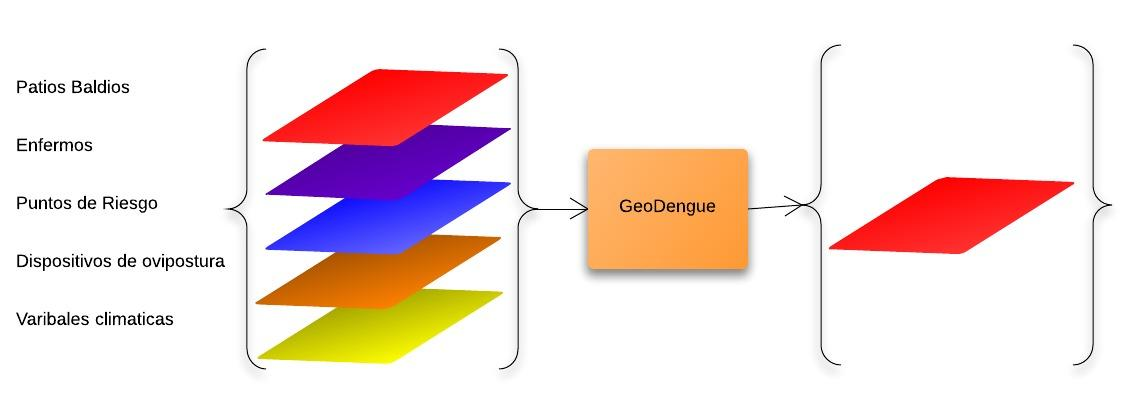
\includegraphics[ scale=0.35]{./graphics/modelo-base.jpeg}
%~ %~
Mediante técnicas de interpolación espacial los datos de entrada serán
procesados y representados en la zona de estudio como polígonos que representan focos de la enfermedad.
%~ %~
Los focos se determina según los valores conocidos de las larvitrampas mediante interpolación, esto representa un instante \cite{AnusuyaSpeech20097}.
 
  %~ * Resultado del conteo de larvas
  %~ * Datos de origen
  %~ * Interpolación
  %~ * Representación
%~ * Predicción de Focos
\section{Proceso Evolutivo}

Se debe explicar lo básico y dar una idea de que se busca y como funciona.


\textbf{Definición 1.} \em Instante \em : Se utiliza el término instante
    para representar a una estrucutra de datos compleja compuesta por
    datos climáticos correspondientes a periodos de tiempos individuales
    $t_{i}$ y otras propiedades complementarias.


\textbf{Definición 2.}\em Peridodo \em : Un periodo es una estrucutra de
    datos que representa a un conjunto de instantes $t_{i}$. El periodo
    $T$ \addsymbol{symbol:P} se define como una colección de $N$ instantes
    $t_{i}$, donde $N$ es el tamaño del periodo de estudio.

    \begin{align*}
        T = t_1,t_2,t_t,\ldots,t_N , & & 1 \leq i \leq N
    \end{align*}


\textbf{Definición 3.} \em Estado \em : Se utliza el término estado
    para representar las etapas del ciclo de desarrollo del \em Aedes Aegypti\em.
    \begin{align*}
        \tau = [huevo, larva, pupa, adulto]
    \end{align*}

\textbf{Definición 4.} \em Sexo \em : Representa el sexo del \em Aedes
    Aegypti\em. Los valores posibles son $MACHO$ y $HEMBRA$.

\textbf{Definición 4.} \em Indiviuduo\em : Se utliza el término individuo
    para representar la unidad del \em Aedes Aegypti \em cualesquiera de sus
    estados, en forma de una estrucutra de datos compleja compuesta de
    propiedades como su madurez y espectativa de vida.

\textbf{Definición 4.} \em Población\em : La población $P$ es una estuctura
    de datos que representa a un grupo de individuos $p_{i}$. Se define como
    una colección de $M$ individuos $p_{i}$, en donde $M$ es el tamaño de
    la población.

    \begin{align*}
        P = p_1,p_2,p_t,\ldots,p_M,  & & 1 \leq i \leq M
    \end{align*}


El proceso evolutivo consiste en somenter los datos, de las muestras obtneidas
mediante la utilización de dispositivos de ovipostura, a las multiples
variaciones climáticas y las caracteristicas biológicas del inividuo.

\section{Consideraciones}
hablar de las consideraciones

Cada $p_{i}$ que pertenzca a $P$ es sometido a las variaciones climáticas de
cada $t_{i}$ que pertenezca a $T$ siempre y cuando $p_{i}$ aún forme parte
de la población $P$.

\section{Operadores básicos}
Durante el proceso evolutivo para cada individuo $p_{j}$ exiten un conjuto
de operadores básicos que son aplicables a todos los individuos sin importar
el sexo y el estado $\tau_{k}$ en el que se encuentre.

hablar de las tablas y la zonificación


\subsection{Madurez}
Para cada $p_{i}$ existe asociado un atributo madurez \addsymbol{symbol:mIi} es
un valor numérico(entre 0 y 100) que varía de acuerdo a las condiciones
climáticas a las que es sometido el mosquito. Cuando la madurez es igual
a 100 el mosquito ya se encuentra listo para un cambio de estado.

\begin{equation}
\eta (t_{i}, p_{j}) = \left\{
  \begin{array}{l l}
    0 & \quad \forall i = 0 \\
    \eta (t_{i-1}, p_{j}) + \frac{1}{\omega(t_{i}) * 24} & \quad \forall i \neq 0
  \end{array} \right.
\end{equation}

\subsection{Cambio de estado}

\begin{equation}
\tau_{k} (t_{i}, p_{j}) = \left\{
  \begin{array}{l l}
    \tau_{k+1} & \quad \forall  \eta(t_{i}, p_{j}) = 100 \\
    \tau_{k} & \quad \text{en caso contrario}
  \end{array} \right.
\end{equation}


\subsection{Mortalidad}
La mortalidad y supervivencia de los individuos se encuentra expresada
mediante la variable de expectativa de vida. La expectativa de vida es
un valor numérico que indica la vitalidad del individuos, esta varía de
acuerdo a las condiciones climáticas a las que es sometido el individuos
durante el proceso evolutivo.

\begin{equation}
\xi (t_{i}, p_{j}) = \left\{
  \begin{array}{l l}
    100 & \quad \forall i = 0 \\
    \xi (t_{i-1}, p_{j}) - \frac{1}{\upsilon(t_{i}) * 24} & \quad \forall i \neq 0
  \end{array} \right.
\end{equation}

El valor de $\xi (t_{i}, p_{j})$ representa el porcentaje de vitalidad del
inidividuo $p_{j}$ luego de ser somenetido a las variaciones del instante
$t_{i}$ perteneciente al periodo $T$ de estudio. La espectativa de vida
para cada individuo $p_{j} \in P$, en el isntante $t_{0}$ se describe como
$\xi (t_{0}, p_{j})= 100$. A medida que $p_{j}$ sea sometido a varios
$t_{i}$ la espectativa de vida irá disminuyendo, si $\xi (t_{i}, p_{j})= 0$ el
idividuo se ha quedado sin espectativa de vida, por lo que se debe proceder
a eliminar $p_{j}$ de $P$ mediante el proceso de reducción de la población
$\theta (t_{i}, p_{j})$.

\begin{equation}
\theta (t_{i}, p_{j}) = \left\{
  \begin{array}{l l}
    p_{j} = null & \quad \xi(t_{i}, p_{j}) == 0 \\
    p_{j} & \quad \text{en caso contrario}
  \end{array} \right.
\end{equation}

\section{Operadores complementarios}
Las etapas inmaduras del \em Aedes Aegigyti\em son principalmente acuaticas
y estaticas, por lo que todas cuentan con caracteristicas similares, no
así la etapa adulto del mosquito que cuenta con ciertas caracteristicas
que divergen mucho del comportamiento básico definido. Debido este
comportamiento especifico todos los $p_{j}$ que se encuentren en el estado
\em Adulto \em cuentan con un conjuto de operadores complementarios que
tienen por objetivo, con ayuda de los operaodres básicos, describir el
comportamiento del mosquito en su estado adulto.

\subsection{Vuelo y búsqueda de alimentos}
Exiten diferencias, en cuanto alimentación y vuelo, entre los adultos
machos y hembras. Los rondan en grupos pequeños o solitariamente,
principalmente atraídos por los mismos huéspedes vertebrados que las hembras.

Las hembras se alimentan principalmente de sangre, que extraen de cualquier
vertebrado, por sus hábitos domésticos muestran marcada predilección por
la del hombre\cite{ThironIzcazaJ2003}. En cuanto a los machos sus partes
bucales no son aptas para chupar sangre, por lo que se alimentan de
carbohidratos de cualquier fuente accesible como frutos o néctar de flores
que satisface sus requerimientos energéticos.

Vuelan en sentido contrario al viento

Por lo general, la hembra de Ae. aegypti no se desplaza más allá de
5,000 m de distancia de radio de vuelo en toda su vida, permanece
físicamente en donde emergió, siempre y cuando no halla algún factor
que la perturbe o no disponga de huéspedes, sitios de reposo y de
postura.


distancia a recorrer
\begin{equation}
 D (t_{i}) = \sqrt{{(\sin(\alpha(t_{i})) * 2000 - S(t_{i}))}^{2}
  + {(\cos(\alpha(t_{i})) * 2000} ^{2} }
\end{equation}
desplazamiento del individuo


\subsection{Reproducción y postura de huevos}



  %~ * Análisis predictivo
  %~ * Descripción del algoritmo de simulación
  %~ * Representación
  %~ * Resultados

%\chapter{Descripción de los algoritmos y modelos utilizados}

\chapter{Resultados y discusión}
%~ * Introducción
%
La población total sobre la cual se realizó el estudio es de 2388 individuos
distribuídos en 85 puntos de control. Cada punto control tiene entre 0 y 133
individuos en el estado larval con edad 0; todas las larvas tienen la misma edad
en el instante inicial de las pruebas.Además, los individuos comparten
las mismas condiciones climáticas, es decir, la temperatura es la misma
para todos los puntos de control \\

\begin{figure}
\centering
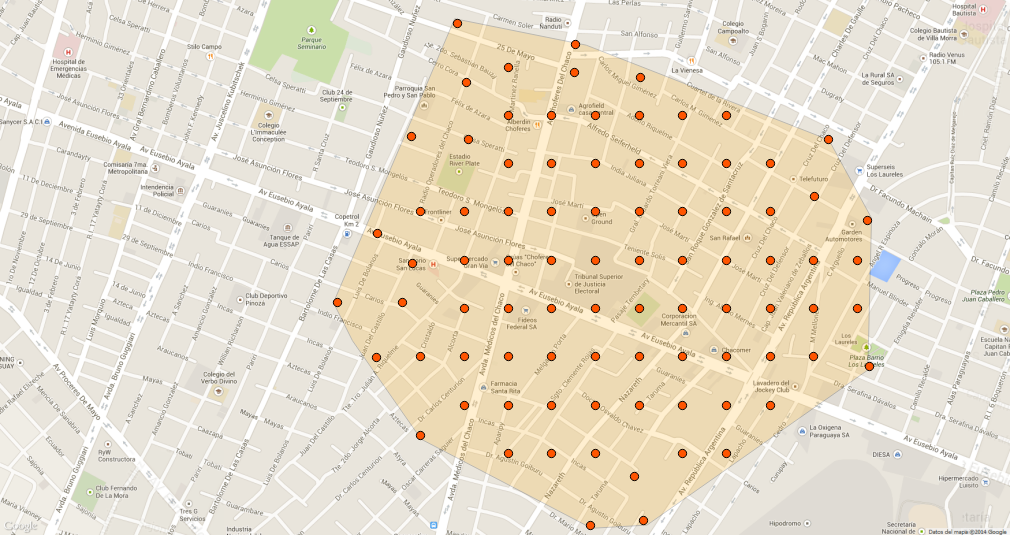
\includegraphics[width=0.9\textwidth]{./capitulo-6/graphics/puntoscontroldistribuido.png}
\caption{\label{fig:distribucion-puntos}Ubicación geográfica y distribución de puntos de control.}
\end{figure}


En la \ref{fig:distribucion-puntos} se observa la distribución de los puntos de control. Geográficamente
corresponde a 4 barrios de la ciudad de Asunción, Paraguay. Los barrios son Nazareth,
Terminal, San Pablo e Hipódromo. Es importante aclarar que la ubicación geográfica
exacta no es relevante para el desarrollo de las pruebas, ya que no se utilizaron
condiciones climáticas propias de dicha ubicación. La ubicación geográfica sirve
de referencia y para poder georeferenciar resultados finales. El área de covertura
es de 2.9$km^2$ y los puntos de control se hallan ubicados uniformemente distribuidos.\\


\begin{table}
    \begin{center}
        \caption{ \label{tab:valores-formulas} Valores de parámetros en fórmulas utilizadas}
        \begin{tabular}{p{3cm} c c c c}
            \hline \\
            Variable & Simbolo & Valor & Fórmula \\
            \hline
            \hline \\
            Sitios de reproducción &  BS & 50 & ver fórmula xxx\\
            Inhibición de eclosión de huevos & $A_{0}$ & 0.5 & ver fórmula xxx\\
        \end{tabular}
    \end{center}
\end{table}

La duración total de días en cada prueba es 50, se toma como día 0 el instante
inicial del proceso evolutivo y como día final al día 49. Para observar la variación
de propiedades biológicas del mosquito Aedes Aegypti se realizaron pruebas a distintas
temperaturas, dichas temperaturas se mantienen constantes durante cada prueba y son las siguientes :
15\textcelsius , 18\textcelsius , 20\textcelsius , 22\textcelsius ,
24\textcelsius , 25\textcelsius , 26\textcelsius , 27\textcelsius ,
30\textcelsius , 34\textcelsius \\


\subsection{Descripción general de las pruebas}

Se realizaron N iteraciones del algoritmo evolutivo y se realizaron las
validaciones sobre el conjunto de datos generado por el mismo

Se presentan los resultados para tasa de desarroollo de las etapas inmaduras
(HUEVO, LARVA y PUPA) del Aedes Aegypti, mortalidad en cada una de las etapas,
la ovipostura, duracion del ciclo gonotrofico, alimentacion, promedio de vuelo y
desplazamiento y distribucion de sexos

\subsection{Tasa de desarollo}
Verificar las tasas de desarrollo de los individuos de la población de forma a validar
si el incremento de la madurez del individuo es correcta. Se debe contar con el tiempo
promedio de de la duración de cada estado, en días, para compararlos con los promedios
generales.

\begin{itemize}
    \item Temperatura constante
    \item Duración en promedio en cada estado a temperatura constante
    \item Desviación estándar
    \item Calcular el error
\end{itemize}

\section{Distribución de Sexo}
Se realizó un análisis para determinar la distribución del sexo del Aedes aegypti. Según
\cite{otero2006stochastic}, alrededor de la mitad de los adultos emergentes son hembras, y se
define una proporción de 1.02:1 macho: hembra. Los autores de \cite{manrique1998desarrollo} la
proporción sexual promedio de adultos emergidos es de $3$ machos por $2,75$ hembras, lo cual no representa una diferencia significativa de una relación 1:1 en las proporciones sexuales.

En general se realizaron pruebas variando la cantidad de individuos de la población, los
resultados se pueden apreciar en la tabla \tabref{tab:distribucion-sexo-test}, donde se observa que
existe una relación 1:1 para la distribución del sexo de los mosquitos.

\begin{table}
    \centering
        \caption{ \label{tab:distribucion-sexo-test} Análisis de la distribución del sexo de Aedes
        aegypti.}
        \begin{tabular}{l c c c }
            \hline \\
            Total de & Adultos & Adultos & Relación \\
            adultos  & machos  & hembras & (macho:hembra) \\
            \hline
            \hline \\
            912    &  461    &  451    &  0,99 : 1,01 \\
            1581   &  812    &  769    &  0,97 : 1,03 \\
            4154   &  2084   &  2070   &  1    : 1 \\
            9722   &  4940   &  4782   &  0,98 : 1,02 \\
            9045   &  4472   &  4573   &  1,01 : 0,99 \\
            16248  &  8104   &  8144   &  1    : 1 \\
            30693  &  15418  &  15275  &  1    : 1 \\
            28411  &  14224  &  14187  &  1    : 1 \\
        \end{tabular}
\end{table}

\section{Ciclo gonotrófico}
Para el análisis de la tasa de desarrollo, en días, del ciclo gonotrófico de las hembras del Aedes
aegypti, se clasificó la población en hembras núliparas y paridas. En la
\tabref{tab:ciclo-gonotrofico-test} se puede observar una media de $5,03$ días para las hembras
nulíparas y  $2,92$ días para las paridas para una temperatura aproximada de $25,11$ \textcelsius.

\begin{table}[!htbp]
    \begin{minipage}{\textwidth}
        \centering
        \caption{ \label{tab:ciclo-gonotrofico-test} Análisis de duración del ciclo gonotrófico
        de la hembra de Aedes aegypti nueve temperaturas constantes  (18-34 \textcelsius).}
        \begin{tabular}{l *{10}{c} }
            \hline \\
            & &  & &  & &  &  &  &  & Media\\
            Población & 18\textcelsius & 20 \textcelsius & 22 \textcelsius & 24 \textcelsius
                      & 25 \textcelsius & 26\textcelsius  & 27 \textcelsius & 30 \textcelsius
                      & 34\textcelsius & General\\

            \hline
            \hline \\
            Nulíparas\footnote{Hembras nulíparas que no han ovipuesto.}
                        & 8,97 & 7,4  & 6,13  & 5,08  & 4,63 & 4,22  & 3,85 & 2,94 & 2,06 & 5,03\\
            Paridas\footnote{Hembras que ya han realizado al menos una ovipostura.}
                        & 5,21 & 4,3  & 3,56  & 2,95  & 2,69 & 2,45  & 2,24 & 1,71 & 1,2 & 2,92\\
            Media \footnote{Promedio general de la duración general del ciclo gonotrófico para las
            hembras}
                        & 7,09 & 5,85 & 4,85  & 4,02  & 3,66 & 3,34  & 3,05 & 2,33 & 1,63 & 3,98\\
        \end{tabular}
    \end{minipage}
\end{table}

Las variaciones en la temperatura influyen en tiempo de digestión de la sangre y el
desarrollo de los ovarios, a medida que la temperatura desciende, la digestión y por ende el ciclo
gonotrófico tomará más tiempo (\figref{fig:ciclo-gonotrofico-temperatura}). En \cite{edman1987host}
se observó que hembras nulíparas de Aedes aegypti poseen un proceso de digestión es más lento en
las hembras paridas y por ende el ciclo gonotrófico de las mismas tiene a ser más largo. Existen
diversos estudios, que han reportado que el patrón diario de alimentación de los mosquitos, varia
de acuerdo a las localidades y subespecies. A continuación se mencionaran algunos estudios
realizados correspondientes a la duración del ciclo gonotrófico, con el fin de realizar una
comparación con los resultados obtenidos mediante el proceso evolutivo.

\begin{figure}[!htbp]
    \centering
    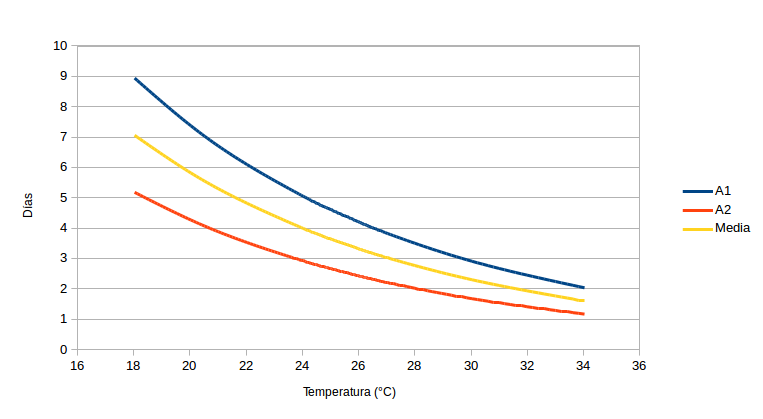
\includegraphics[width=1\textwidth]{capitulo-6/graphics/ciclo-gonotrofico-temperatura.png}
    \caption{\label{fig:ciclo-gonotrofico-temperatura} Tasa de desarrollo, en días, del ciclo
    gonotrófico de hembras nulíparas, hembras paridas y la media general a nueve temperaturas
    constantes (18-34 \textcelsius).}
\end{figure}

En \cite{beltran2001bionomia} se determinó que la duración del ciclo gonotrófico del Aedes
aegypti, para los siguientes municipios de México en, 3 días para Tamazula de Gordiano a una
temperatura de $21,5$ \textcelsius, 3 días para Techaluta de Montenegro a $22,8$ \textcelsius, 4
días para Tuxpan a 22 \textcelsius y 5 días para CD Zacoalco de Torres a $22,7$ \textcelsius.

En \cite{luevano1993ciclo}, el autor determinó la duración del ciclo gonotrófico de las
poblaciones naturales de Aedes aegypti en el área metropolitana de Monterrey, Nuevo León. México,
en cinco días, a una temperatura promedio de $25,5$ \textcelsius.

En \cite{trpis1986dispersal} los autores reportaron una duración del ciclo gonotrófico en Kenia a
nivel rural de, 5 a 7 días para el primer ciclo (hembras nulíparas) y de 4 a 5 días para los
siguientes ciclos (hembras paridas). El método utilizado fue de captura con cebo humano de
mosquitos de Aedes aegypti.

Según \cite{sivanathan2006ecology} el ciclo gonotrófico del aAedes aegypti y Aedes albopictus se
encuentra acotada entre $2,73$ a 3 días respectivamente.

Las diferentes condiciones climáticas y la capacidad de adaptación en habitad específicos, del
Aedes aegypti, son las responsables de diferencias que se puedan tener entre cepas del mosquito.
La duración del ciclo gonotrófico obtenida, depende de los coeficientes para el modelo de
maduración enzimática de \cite{sharpe1977reaction} que fue tomado de \cite{otero2006stochastic},
que según los autores fue tomado de \cite{focks1993dynamic}.


\section{Ovoposturas}
Como se menciona en la la sección \ref{subsec:cap4-oviposicion} la cantidad de huevos generados,
por una hembra, se encuentra definida como una constante independiente de la temperatura temperatura de valor 63. En la tabla
\ref{tab:ovipostura-cantidad-test} se presentan los resultados obtenidos de la cantidad de
huevos generados. En general fueron generados 747739 huevos por 11708 hembras adultas dejando
un promedio de 63.87 huevos por hembra, dejando un error 0.87 huevos.

\begin{table}
    \begin{center}

        \caption{ \label{tab:ovipostura-cantidad-test} Análisis de la
        cantidad de huevos de Aedes Aegypti generados a diez temperaturas
        constantes  (15-34 \textcelsius).}
        \begin{tabular}{p{3cm} c c  }
            \hline \\
            Temperatura  & Cantidad          & Cantidad \\
            \textcelsius & de oviposiciones  & de huevos \\
            \hline
            \hline \\
                15 & 0    & 0\\
                18 & 44   & 2772\\
                20 & 91   & 5733\\
                22 & 119  & 7497\\
                24 & 431  & 27153\\
                25 & 810  & 51030\\
                26 & 1003 & 63189\\
                27 & 1185 & 74655\\
                30 & 5206 & 327978\\
                34 & 2058 & 129654\\

        \end{tabular}
    \end{center}
\end{table}


\section{Vuelo y dispersión}
Para el análisis de la distancia recorrida, en metros, del adulto de Aedes aegypti, se realizaron
pruebas a 9 temperaturas constantes (15-34\textcelsius), solo las hembras que han ovipuesto al
menos una vez fueron incluidas. En la tabla \ref{tab:pomedio-vuelo-test} se presentan los
resultados obtenidos para la disperción de las hembras adultas del aedes aegypit agrupadas por el
tipo su tipo de zona, en general se obtuvo un promedio de $65,74$, $63,97$ $1308,19$ metros para las zonas buena, normal y malas respectivamente. Existen diversos estudios, que han reportado que
la disperción del aedes aegypti en relación a las caracteristicas de su ambiente. A continuación
se mencionaran algunos estudios realizados, con el fin de realizar una comparación con los resultados obtenidos.

En \cite{cabezas2005dengue} señalan que por lo general mosquito no sobrepasa los 50 a 100 metros
durante su vida, ya que tiende a permanecer en el lugar donde emergió.

Según \cite{ThironIzcazaJ2003} por lo general, la hembra de Ae. aegypti, permanece físicamente en
donde emergió, siempre y cuando no halla algún factor que la perturbe o no disponga de huéspedes,
sitios de reposo y de postura. En caso de no haber recipientes adecuados, la hembra grávida es capaz de volar hasta tres kilómetros en busca de este sitio.

Los autores de \cite{dengueUruguayCap8} señalan que, para las estrategias de control de Aedes
aegypti en zonas urbanas donde existen brotes de dengue y fiebre amarilla se asume que los
mosquitos tienen un rango de vuelo durante su vida de 50 a 100 metros.

En \cite{luevano1993ciclo} se reporta, que el aedes aegypti es un mosquito doméstico que
generalmente esta confinado a las casas donde se cria, tiene un rango de vuelo corto, entre 23 a 50 metros, y raramente se dispersa a largas distancias.

\cite{mcdonald1977population} en Kenia, liberó poblaciones de Aedes aegypti a las distancias de,
200, 400 y 800 metros, y observó que aproximadamente el 50 \% de los mosquitos marcados se
dispersaron a 200 metros del punto en el cual fueron liberados, un 10 \% a 400 metros y solamente
el 1 \% se dispersó a 800 metros.

En \cite{trpis1986dispersal}, los autores reportaron que en Kenia, que la tasa media de dispersión
de las hembras fue de 57 metros. La distancia máxima de las hembras durante 24 horas fue de 154
metros.

La mayoría de los estudios coinciden que, los adultos del aedes aegypti, en condiciones óptimas de
disponibilidad de alimento y sitios adecuados de ovipostura, tienden a permanecer en el lugar
donde emergieron, con una dispersión media estimada entre 50 y a 100 metros, su presencia es
prácticamente un indicio certero de la proximidad de los criaderos. En caso de no contar con
sitios adecuados de ovipostura y disponibilidad de alimento tienden a dispersarme una mayor
distancia en busca de mejores condiciones.

\begin{table}
    \begin{minipage}{\textwidth}
        \caption{ \label{tab:pomedio-vuelo-test} Análisis de la dispersión, por zona, del adulto
        de Aedes aegypti diez temperaturas constantes (15-34 \textcelsius).}
        \begin{tabular}{p{4cm} *{4}{c}  }
          \hline \\
          Temperatura (\textcelsius)& Buena & Normal & Mala & Media Obtenida\\
          \hline
          \hline \\
          18 & 89,06 & 66,61 & 1274,97 & 476,88\\
          20 & 66,52 & 73,53 & 1516,43 & 552,16\\
          22 & 77,89 & 63,78 & 1003,9 & 381,86\\
          24 & 60,28 & 62,31 & 1077,6 & 400,06\\
          25 & 54,52 & 63,66 & 1397,31 & 505,16\\
          26 & 61,61 & 60,79 & 1509,67 & 544,02\\
          27 & 65,24 & 63,72 & 1433,58 & 520,85\\
          30 & 62,61 & 59,56 & 1213,1 & 445,09\\
          34 & 53,92 & 61,75 & 1347,13 & 487,6\\
          Media General & 65,74 & 63,97 & 1308,19 & 479,3\\
        \end{tabular}
    \end{minipage}
\end{table}




\subsection{Tasa de desarollo}
Verificar las tasas de desarrollo de los individuos de la población de forma a validar
si el incremento de la madurez del individuo es correcta. Se debe contar con el tiempo
promedio de de la duración de cada estado, en días, para compararlos con los promedios
generales.

\begin{itemize}
    \item Temperatura constante
    \item Duración en promedio en cada estado a temperatura constante
    \item Desviación estándar
    \item Calcular el error
\end{itemize}

\section{Ciclo gonotrófico}
Para el análisis de la tasa de desarrollo, en días, del ciclo gonotrófico de las hembras del Aedes
aegypti, se clasificó la población en hembras núliparas y paridas. En la
\tabref{tab:ciclo-gonotrofico-test} se puede observar una media de $5,03$ días para las hembras
nulíparas y  $2,92$ días para las paridas para una temperatura aproximada de $25,11$ \textcelsius.

\begin{table}[!htbp]
    \begin{minipage}{\textwidth}
        \centering
        \caption{ \label{tab:ciclo-gonotrofico-test} Análisis de duración del ciclo gonotrófico
        de la hembra de Aedes aegypti nueve temperaturas constantes  (18-34 \textcelsius).}
        \begin{tabular}{l *{10}{c} }
            \hline \\
            & &  & &  & &  &  &  &  & Media\\
            Población & 18\textcelsius & 20 \textcelsius & 22 \textcelsius & 24 \textcelsius
                      & 25 \textcelsius & 26\textcelsius  & 27 \textcelsius & 30 \textcelsius
                      & 34\textcelsius & General\\

            \hline
            \hline \\
            Nulíparas\footnote{Hembras nulíparas que no han ovipuesto.}
                        & 8,97 & 7,4  & 6,13  & 5,08  & 4,63 & 4,22  & 3,85 & 2,94 & 2,06 & 5,03\\
            Paridas\footnote{Hembras que ya han realizado al menos una ovipostura.}
                        & 5,21 & 4,3  & 3,56  & 2,95  & 2,69 & 2,45  & 2,24 & 1,71 & 1,2 & 2,92\\
            Media \footnote{Promedio general de la duración general del ciclo gonotrófico para las
            hembras}
                        & 7,09 & 5,85 & 4,85  & 4,02  & 3,66 & 3,34  & 3,05 & 2,33 & 1,63 & 3,98\\
        \end{tabular}
    \end{minipage}
\end{table}

Las variaciones en la temperatura influyen en tiempo de digestión de la sangre y el
desarrollo de los ovarios, a medida que la temperatura desciende, la digestión y por ende el ciclo
gonotrófico tomará más tiempo (\figref{fig:ciclo-gonotrofico-temperatura}). En \cite{edman1987host}
se observó que hembras nulíparas de Aedes aegypti poseen un proceso de digestión es más lento en
las hembras paridas y por ende el ciclo gonotrófico de las mismas tiene a ser más largo. Existen
diversos estudios, que han reportado que el patrón diario de alimentación de los mosquitos, varia
de acuerdo a las localidades y subespecies. A continuación se mencionaran algunos estudios
realizados correspondientes a la duración del ciclo gonotrófico, con el fin de realizar una
comparación con los resultados obtenidos mediante el proceso evolutivo.

\begin{figure}[!htbp]
    \centering
    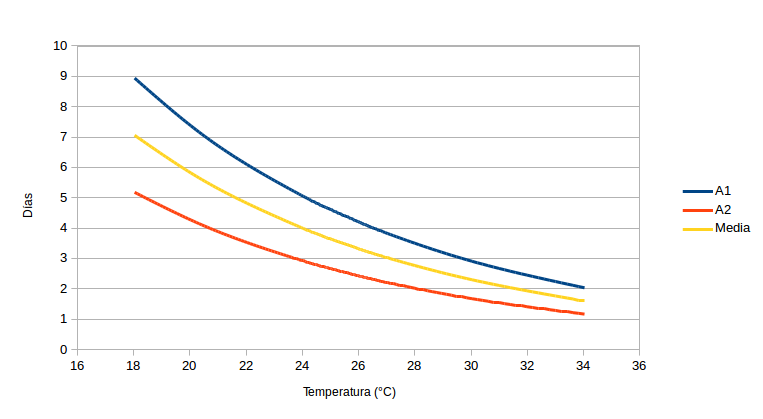
\includegraphics[width=1\textwidth]{capitulo-6/graphics/ciclo-gonotrofico-temperatura.png}
    \caption{\label{fig:ciclo-gonotrofico-temperatura} Tasa de desarrollo, en días, del ciclo
    gonotrófico de hembras nulíparas, hembras paridas y la media general a nueve temperaturas
    constantes (18-34 \textcelsius).}
\end{figure}

En \cite{beltran2001bionomia} se determinó que la duración del ciclo gonotrófico del Aedes
aegypti, para los siguientes municipios de México en, 3 días para Tamazula de Gordiano a una
temperatura de $21,5$ \textcelsius, 3 días para Techaluta de Montenegro a $22,8$ \textcelsius, 4
días para Tuxpan a 22 \textcelsius y 5 días para CD Zacoalco de Torres a $22,7$ \textcelsius.

En \cite{luevano1993ciclo}, el autor determinó la duración del ciclo gonotrófico de las
poblaciones naturales de Aedes aegypti en el área metropolitana de Monterrey, Nuevo León. México,
en cinco días, a una temperatura promedio de $25,5$ \textcelsius.

En \cite{trpis1986dispersal} los autores reportaron una duración del ciclo gonotrófico en Kenia a
nivel rural de, 5 a 7 días para el primer ciclo (hembras nulíparas) y de 4 a 5 días para los
siguientes ciclos (hembras paridas). El método utilizado fue de captura con cebo humano de
mosquitos de Aedes aegypti.

Según \cite{sivanathan2006ecology} el ciclo gonotrófico del aAedes aegypti y Aedes albopictus se
encuentra acotada entre $2,73$ a 3 días respectivamente.

Las diferentes condiciones climáticas y la capacidad de adaptación en habitad específicos, del
Aedes aegypti, son las responsables de diferencias que se puedan tener entre cepas del mosquito.
La duración del ciclo gonotrófico obtenida, depende de los coeficientes para el modelo de
maduración enzimática de \cite{sharpe1977reaction} que fue tomado de \cite{otero2006stochastic},
que según los autores fue tomado de \cite{focks1993dynamic}.


\section{Vuelo y dispersión}
Para el análisis de la distancia recorrida, en metros, del adulto de Aedes aegypti, se realizaron
pruebas a 9 temperaturas constantes (15-34\textcelsius), solo las hembras que han ovipuesto al
menos una vez fueron incluidas. En la tabla \ref{tab:pomedio-vuelo-test} se presentan los
resultados obtenidos para la disperción de las hembras adultas del aedes aegypit agrupadas por el
tipo su tipo de zona, en general se obtuvo un promedio de $65,74$, $63,97$ $1308,19$ metros para las zonas buena, normal y malas respectivamente. Existen diversos estudios, que han reportado que
la disperción del aedes aegypti en relación a las caracteristicas de su ambiente. A continuación
se mencionaran algunos estudios realizados, con el fin de realizar una comparación con los resultados obtenidos.

En \cite{cabezas2005dengue} señalan que por lo general mosquito no sobrepasa los 50 a 100 metros
durante su vida, ya que tiende a permanecer en el lugar donde emergió.

Según \cite{ThironIzcazaJ2003} por lo general, la hembra de Ae. aegypti, permanece físicamente en
donde emergió, siempre y cuando no halla algún factor que la perturbe o no disponga de huéspedes,
sitios de reposo y de postura. En caso de no haber recipientes adecuados, la hembra grávida es capaz de volar hasta tres kilómetros en busca de este sitio.

Los autores de \cite{dengueUruguayCap8} señalan que, para las estrategias de control de Aedes
aegypti en zonas urbanas donde existen brotes de dengue y fiebre amarilla se asume que los
mosquitos tienen un rango de vuelo durante su vida de 50 a 100 metros.

En \cite{luevano1993ciclo} se reporta, que el aedes aegypti es un mosquito doméstico que
generalmente esta confinado a las casas donde se cria, tiene un rango de vuelo corto, entre 23 a 50 metros, y raramente se dispersa a largas distancias.

\cite{mcdonald1977population} en Kenia, liberó poblaciones de Aedes aegypti a las distancias de,
200, 400 y 800 metros, y observó que aproximadamente el 50 \% de los mosquitos marcados se
dispersaron a 200 metros del punto en el cual fueron liberados, un 10 \% a 400 metros y solamente
el 1 \% se dispersó a 800 metros.

En \cite{trpis1986dispersal}, los autores reportaron que en Kenia, que la tasa media de dispersión
de las hembras fue de 57 metros. La distancia máxima de las hembras durante 24 horas fue de 154
metros.

La mayoría de los estudios coinciden que, los adultos del aedes aegypti, en condiciones óptimas de
disponibilidad de alimento y sitios adecuados de ovipostura, tienden a permanecer en el lugar
donde emergieron, con una dispersión media estimada entre 50 y a 100 metros, su presencia es
prácticamente un indicio certero de la proximidad de los criaderos. En caso de no contar con
sitios adecuados de ovipostura y disponibilidad de alimento tienden a dispersarme una mayor
distancia en busca de mejores condiciones.

\begin{table}
    \begin{minipage}{\textwidth}
        \caption{ \label{tab:pomedio-vuelo-test} Análisis de la dispersión, por zona, del adulto
        de Aedes aegypti diez temperaturas constantes (15-34 \textcelsius).}
        \begin{tabular}{p{4cm} *{4}{c}  }
          \hline \\
          Temperatura (\textcelsius)& Buena & Normal & Mala & Media Obtenida\\
          \hline
          \hline \\
          18 & 89,06 & 66,61 & 1274,97 & 476,88\\
          20 & 66,52 & 73,53 & 1516,43 & 552,16\\
          22 & 77,89 & 63,78 & 1003,9 & 381,86\\
          24 & 60,28 & 62,31 & 1077,6 & 400,06\\
          25 & 54,52 & 63,66 & 1397,31 & 505,16\\
          26 & 61,61 & 60,79 & 1509,67 & 544,02\\
          27 & 65,24 & 63,72 & 1433,58 & 520,85\\
          30 & 62,61 & 59,56 & 1213,1 & 445,09\\
          34 & 53,92 & 61,75 & 1347,13 & 487,6\\
          Media General & 65,74 & 63,97 & 1308,19 & 479,3\\
        \end{tabular}
    \end{minipage}
\end{table}

\section{Distribución de Sexo}
Se realizó un análisis para determinar la distribución del sexo del Aedes aegypti. Según
\cite{otero2006stochastic}, alrededor de la mitad de los adultos emergentes son hembras, y se
define una proporción de 1.02:1 macho: hembra. Los autores de \cite{manrique1998desarrollo} la
proporción sexual promedio de adultos emergidos es de $3$ machos por $2,75$ hembras, lo cual no representa una diferencia significativa de una relación 1:1 en las proporciones sexuales.

En general se realizaron pruebas variando la cantidad de individuos de la población, los
resultados se pueden apreciar en la tabla \tabref{tab:distribucion-sexo-test}, donde se observa que
existe una relación 1:1 para la distribución del sexo de los mosquitos.

\begin{table}
    \centering
        \caption{ \label{tab:distribucion-sexo-test} Análisis de la distribución del sexo de Aedes
        aegypti.}
        \begin{tabular}{l c c c }
            \hline \\
            Total de & Adultos & Adultos & Relación \\
            adultos  & machos  & hembras & (macho:hembra) \\
            \hline
            \hline \\
            912    &  461    &  451    &  0,99 : 1,01 \\
            1581   &  812    &  769    &  0,97 : 1,03 \\
            4154   &  2084   &  2070   &  1    : 1 \\
            9722   &  4940   &  4782   &  0,98 : 1,02 \\
            9045   &  4472   &  4573   &  1,01 : 0,99 \\
            16248  &  8104   &  8144   &  1    : 1 \\
            30693  &  15418  &  15275  &  1    : 1 \\
            28411  &  14224  &  14187  &  1    : 1 \\
        \end{tabular}
\end{table}


%\chapter{Conclusiones y Trabajos Futuros}

%\chapter{Trabajos Futuros}




\appendix   % inician los apendices de tu tesis
% los cap'itulos que incluyas a partir de aqu'i aparecen
% como ap'endices
%\chapter{Especificaciones de dispositivos de ovipostura}

\section{Larvitrampas}

\subsection{Especificaciones para la colocación e inspección}
Instalarla a una altura de 50 cm (del suelo a la base de la larvitrampa). Protegerla de la luz
directa del sol, el aire, la lluvia, en lugares a media luz o completamente a la sombra. No deben
ubicarse cercanas a depósitos de agua. Debe evitarse su colocación en lugares completamente
pavimentados, u otros que tengan mucha refracción de la luz. Debe estar visible para la
hembra del mosquito. Protegerla de niños y animales domésticos (perros, gatos, roedores, etc.).

Un prerrequisito para cualquier tipo de larvitrampa en secciones de llantas es que facilite la
inspección visual del agua insitu o que transfiera fácilmente los contenidos a otro recipiente
para que sean examinados.

\subsection{Forma de revisión}
Se establece una rutina semanal para revisar las larvitrampas, para lo cual, una vez por semana
debe vaciarse todo su contenido cuidadosamente (para que no quede ninguna larva en sus paredes) en
un recipiente adecuado para realizar la inspección. En caso de ser positivas, se registra como tal
y las larvas serán colectadas en tubos para ser enviadas al laboratorio para su determinación
taxonómica. Luego, el dispositivo se lava y se acondiciona para ser colocadas nuevamente siguiendo
las especificaciones ya descritas.

Antes de la utilización de la larvitrampa, ésta debe cepillarse y flamearse, luego mantenerla
sumergida en agua durante no menos de tres días, para asegurarse que el agua no contenga residuos
de sustancias que puedan actuar como larvicida. De esta manera, además, se garantiza la
destrucción de algún huevo del mosquito que estuviese previamente en el neumático o en
larvitrampas ya utilizadas.

\subsection{Consideración final}


Tener en cuenta que en verano, con condiciones más favorables para el desarrollo de esta especie,
las larvas pueden alcanzar el estadio de adulto entre 6 y 7 días desde la ovipostura, por lo que
es necesaria la inspección de todas las larvitrampas en los tiempos indicados a fin de evitar que
alguna de ellas se transformen en criaderos de adultos.

\section{Ovitrampa}

\subsection{Especificaciones para la colocación e inspección}
La colocación debe realizarse en lugares representativos del municipio,
especialmente en las zonas donde se produjeron casos de dengue autóctonos
o importados. Respecto al número de ovitrampas a colocar, se sugiere no
menor a 10 por localidad. La idea es mantener el mismo circuito (mismos
lugares de colocación), un modelo a “escala ciudad”, para tener la idea de
la "presencia" relacionada con la distribución geográfica del vector, se
basa en el criterio que la información sea independiente. O sea que sea
improbable (más bien imposible) que una hembra pueda poner huevos en dos
ovitrampas contiguas. Además la instalación debería basarse en la capacidad
operativa de trabajo, y para ello se pueden colocar las ovitrampas en una
grilla con puntos más o menos equidistantes de aproximadamente 400 metros
de lado.

Cada ovitrampa se coloca en un lugar accesible, protegido donde predomine
la sombra y haya cierto grado de humedad (ambiente sombreado). Debe asegurarse
la presencia de moradores al retirarla.Sobre un plano de la localidad o
sector a muestrear se seleccionarán los puntos donde se colocarán las
ovitrampas. Una variante sería colocar una por Unidad Sanitaria que el
municipio posea, asumiendo que la ubicación de las mismas brindará una
visión representativa del conjunto. Conviene tener presente que en este
caso, el muestreo puede no ser representativo de viviendas regulares.

Las ovitrampas deben ser inspeccionadas semanalmente y en el caso de detectar
paletas con huevos, cuando no puedan ser leídos en el nivel local, se deberán
remitir para su lectura a los laboratorios de entomología más cercanos,
(Divisiones de Zoonosis Urbanas, División de Zoonosis Rurales, CEPAVE, etc.).
La remisión será en un sobre o bolsita plástica, con los datos para georreferenciar.
La vigilancia entomológica se debe realizar en forma continua anual. Es
importante destacar que una vez detectada la presencia de Aedes Aegypti por
cualquiera de los sistemas de monitoreo (larvitrampas u ovitrampas) se deben
realizar las acciones inmediatas de control focal en la comunidad.

\subsection{Consideración final}
Es importante añadir un identificador a cada ovitrampa que permita la
identificarlas fácilmente. El rótulo se debe colocar sobre la baja-lengua
o paleta de la ovitrampa, debe estar debidamente escrito (con lápiz) el
número y/o código de la ovitrampa. También se rotulará el frasco sobre
su pared con tinta indeleble. Se recomienda numerar cada una de las paletas
o baja-lenguas y agregarle iniciales para identificar el municipio y
detallar en el protocolo común los datos de cada una (lugar físico por.
ej. calle, barrio y zona del municipio como también la fecha del retiro
de las mismas de su lugar para su posterior envío).

\section{Mosquitérica genérica}

Los materiales para la construcción son los siguientes :
\begin{itemize}
    \item Una botella de plástico de 2 litros.
    \item Tijeras.
    \item Una lija para madera.
    \item Un rollo de cinta aislante.
    \item Una pieza de tul o gasa para sellar la boquilla (cuello).
    \item Un poco de arroz o alpiste.
    \item 250 ml de agua no clorada.
\end{itemize}

Hay que cortar el cilindro en dos partes, de modo que la porción de la
boca quede en forma contraria, formando un embudo. Debe retirarse el tapón
de la botella. Asimismo, se debe retirar con cuidado el anillo de precinto
y almacenarlo, también se utilizará en la mosquitérica.

Se debe lijar bien dentro del "embudo". Esto servirá para aumentar el área
de evaporación, y será más fácil para el mosquito localizar la  trampa.
Hay que colocar la  tela en el cuello y asegurarlo con el anillo. Hay que
tener en cuenta que debe existir un tejido muy fino, de modo que las larvas
no puedan pasar;


Hay que colocar en la parte inferior de la botella la comida que se eligió,
puede ser granos de alpiste o tres granos de arroz, pero siempre triturados.
Se inserta la porción de cuello hacia abajo sobre la parte inferior de la
botella; Se usa cinta adhesiva para asegurar las dos partes, sobre el lado
exterior.

Se pone el agua sin cloro en la mosquitérica a pocos centímetros por encima
del cuello. Si no dispone de agua sin cloro, se usa agua de tomar del grifo
y se deja que repose durante dos días.

\subsection{Especificaciones para la colocación e inspección}
Las técnicas de colocación e inspección mencionadas anteriormente se aplican
a este método.

\subsection{Consideración final}
Actualmente la mosquitérica es utilizada en reemplazo a los antiguos
dispositivos de ovipostura en los últimos trabajos realizados en sudamérica
para el control del vector del dengue por presentar resultados más exactos.

% estos comandos generan la bilbiograf'ia
\printbibliography

\end{document}
